\documentclass[14pt]{article}
\usepackage[utf8]{inputenc}
\usepackage[spanish]{babel}
\usepackage[margin=3cm]{geometry}
\usepackage{graphicx}
\usepackage{wrapfig}
\usepackage{fancyhdr}
\usepackage{hyperref}

\title{ESCOMMERCE}

\renewcommand{\headrulewidth}{0pt}
\cfoot[]{}
\rfoot[]{Fecha Límite de Entrega: Miércoles 18 de Mayo del 2021}

\pagestyle{fancy}

\begin{document}
    \begin{center}

        \begin{figure}[htbl!]
            \begin{minipage}[b]{0.5\linewidth}
                
\includegraphics[height=0.4\textwidth]{IPN.jpg}
                \label{fig:IPN}
            \end{minipage}
            \hspace{2.5cm}
            \begin{minipage}[b]{0.5\linewidth}
                \centering
                
\includegraphics[height=0.4\textwidth]{ESCOM.png}
                \label{fig:ESCOM}
            \end{minipage}
        \end{figure}

        \vspace{1cm}

        \fontsize{14}{baseline skip}\textbf{INSTITUTO POLITÉCNICO NACIONAL \\
        \vspace{0.3cm}ESCUELA SUPERIOR DE CÓMPUTO}

        \vspace{3cm}

        \fontsize{14}{baseline skip} ANÁLISIS Y DISEÑO ORIENTADO A OBJETOS\\ \vspace{0.5cm}MALDONADO CASTILLO IDALIA\\ \vspace{0.5cm}2CV17

        \vspace{3cm}

        \fontsize{14}{baseline skip}Escobar Armenta Jacqueline\\
        \vspace{0.3cm}Hernández Cárdenas Daniel\\
        \vspace{0.3cm}Martínez Alvarado José Iván\\
        \vspace{0.3cm}Osorio Garcia Daniel Alejandro\\
        \vspace{0.3cm}Ramírez Guerrero Jessica\\
        \vspace{0.3cm}Rojas Hernández Johan Ali\\
        \vspace{0.3cm}Vargas Medina Miguel Angel\\
        \vspace{0.3cm}Zuñiga Mendoza Carlos Jafeth

    \end{center}

    \newpage
    \cfoot[]{\thepage}
    \rfoot[]{}
    \large
    

    \addtocontents{toc}{\hspace{-7.5mm} \textbf{Capítulos}}
    \addtocontents{toc}{\hfill \textbf{Página} \par}
    \addtocontents{toc}{\vspace{-2mm} \hspace{-7.5mm} \hrule \par}

    \newpage
    \tableofcontents
    
    \vspace{0.5cm}
    \maketitle
    \section{Introducción}
        \subsection{Objetivo}
        
        \begin{quote}
            ESCOMMERCE, tiene como objetivo principal impulsar el comercio electrónico o e-commerce dentro de la comunidad de ESCOM. 
            
            \vspace{0.5cm}Esto con la finalidad de impulsar este medio de distribución y la economía de los interesados sin importar si son estudiantes, docentes o personal.
    
            \vspace{0.5cm}Los productos ofertados dentro de la plataforma deberán de cumplir con las siguientes normas:
            
                \begin{itemize}
                    \item Se debe comprobar la legalidad del artículo
                    \item Las condiciones óptimas para la venta
                    \item Indicar el stock disponible para venta
                    \item Mayor de edad
                    \item Confirmar que eres parte de la comunidad de ESCOM
                \end{itemize}
    
            \vspace{0.5cm}El usuario tendrá la posibilidad de realizar compra y venta de productos. Estos productos se clasifican según sus características y descripciones esenciales, delimitadas por las necesidades de la comunidad.
    
            \vspace{0.5cm}Cuando el usuario desee realizar una compra, esta estará denotada por un número de serie o de seguimiento único.
    
            \vspace{0.5cm}Para poder realizar la entrega del producto el usuario dispondrá de dos métodos, en caso de envío tendrá que brindar ciertos datos a nuestro software, estos datos estarán resguardados por las leyes correspondientes de confidencialidad. En caso de solicitar recoger en punto de recolección, tendrá que seleccionar alguno de los centros ubicados dentro del plantel.
    
            \vspace{0.5cm}Una vez realizada la entrega del producto, dependiendo de la clasificación del producto, el usuario dispone de un número establecido de días para solicitar un reembolso o reposición del producto. En caso de solicitar una reposición el usuario deberá adjuntar pruebas sobre las condiciones del producto con una breve descripción del problema para continuar el proceso de validación.
    
            \vspace{0.5cm}La plataforma será desarrollada de la siguiente forma:
    
            \vspace{0.5cm}Frontend: JavaScript, HTML,CSS 
    
            \vspace{0.5cm}Backend: Python, MySQL
    
            \vspace{0.5cm}Nuestra página no se hace responsable por las condiciones de los productos ofertados después del tiempo estipulado de garantía, el cliente acepta estos riesgos
        \end{quote}
        
        \subsection{Limitantes}
            \begin{itemize}
                \item Tiempos de entrega reducidos
                \item Falta de compromiso por parte de algunos integrantes
                \item Falta de dominio en algunas de las tecnologías implementadas
                \item Recursos de hardware para un óptimo desarrollo
                \item Disponibilidad de tiempos debido a la carga de trabajo de materias
                \item Desconfianza por parte de los usuarios 
            \end{itemize}
        
        \subsection{Objetivo General}
            \begin{quote}
                Implementar una nueva plataforma mediante la cual se motive a la comunidad a introducirse en el e-commerce.
            \end{quote}
        
    \section{Modelo de Negocios}
        \subsection{Requerimientos funcionales}
            \begin{quote}
                \subsubsection{RF1 Crear cuenta}\label{RF1 Crear cuenta}
                    \begin{quote}
                        Tipo: Requerimiento
                        
                        Nivel: Obligatorio
                        
                        Estado: Propuesta
                        
                        Descripción: Dentro del sistema las personas podrán crear una cuenta con los campos requeridos.
                    \end{quote}
                \subsubsection{RF2 Visualizar información}\label{RF2 Visualizar información}
                    \begin{quote}
                        Tipo: Requerimiento
                        
                        Nivel: Obligatorio
                        
                        Estado: Propuesta
                        
                        Descripción: El sistema le permitirá al usuario ver la información almacenada en su cuenta.
                    \end{quote}
                \subsubsection{RF3 Actualizar información de la cuenta}\label{RF3 Actualizar información de la cuenta}
                    \begin{quote}
                        Tipo: Requerimiento
                        
                        Nivel: Obligatorio
                        
                        Estado: Propuesta
                        
                        Descripción: Dentro del sistema el usuario podrá actualizar los datos básicos de su cuenta, en caso de que así lo requiera.
                    \end{quote}
                \subsubsection{RF4 Eliminar cuenta}\label{RF4 Eliminar cuenta}
                    \begin{quote}
                    Tipo: Requerimiento
                    
                    Nivel: Obligatorio
                    
                    Estado: Propuesta
                    
                    Descripción: Dentro del sistema el usuario podrá eliminar su cuenta, en caso de que así lo requiera.
                    \end{quote}
                \subsubsection{RF5 Ingresar al sistema}\label{RF5 Ingresar al sistema}
                    \begin{quote}
                        Tipo: Requerimiento
                        
                        Nivel: Obligatorio
                        
                        Estado: Propuesta
                        
                        Descripción: Dentro del sistema el usuario podrá iniciar sesión con las credenciales correspondientes a su cuenta
                    \end{quote}
                \subsubsection{RF6 Publicar producto}\label{RF6 Publicar producto}
                    \begin{quote}
                        Tipo: Requerimiento
                        
                        Nivel: Obligatorio
                        
                        Estado: Propuesta
                        
                        Descripción: El usuario será capaz de subir al sistema el producto que pondrá en venta para los demás usuarios.
                    \end{quote}
                \subsubsection{RF7 Buscar  productos}\label{RF7 Buscar  productos}
                    \begin{quote}
                        Tipo: Requerimiento
    
                        Nivel: Obligatorio
    
                        Estado: Propuesta
    
                        Descripción: Dentro del sistema se contará con una barra de búsqueda que permitirá explorar libremente los productos del catálogo, solo mostrará productos que cumplan con los criterios seleccionados.
                    \end{quote}
                \subsubsection{RF8 Separar por categorías}\label{RF8 Separar por categorías}
                    \begin{quote}
                        Tipo: Requerimiento
                        
                        Nivel: Obligatorio
                        
                        Estado: Propuesta
                        
                        Descripción: El sistema permitirá al cliente navegar a través de las categorías de productos.
                    \end{quote}
                \subsubsection{RF9 Filtrar por categorías}\label{RF9 Filtrar por categorías}
                    \begin{quote}
                        Tipo: Requerimiento
                        
                        Nivel: Obligatorio
                        
                        Estado: Propuesta
                        
                        Descripción: El sistema permite al comprador depurar su búsqueda entre los distintos productos por marca o rango de precio.
                    \end{quote}
                \subsubsection{RF10 Agregar al carrito}\label{RF10 Agregar al carrito}
                    \begin{quote}
                        Tipo: Requerimiento
                        
                        Nivel: Obligatorio
                        
                        Estado: Propuesta
                        
                        Descripción: Dentro del sistema un cliente podrá seleccionar un producto y añadirlo al carrito de compra. En el carrito se podrán agregar artículos o eliminar los artículos previamente seleccionados.
                    \end{quote}
                \subsubsection{RF11 Notificar usuario}\label{RF11 Notificar usuario}
                    \begin{quote}
                        Tipo: Requerimiento
                        
                        Nivel: Obligatorio
                        
                        Estado: Propuesta
                        
                        Descripción: El sistema enviará un mensaje de confirmación cuando un usuario se da de alta por primera vez, cuando realice un pedido de venta, cuando se pongan a la venta productos, cuando se verifique el pago de un producto y cuando se apruebe una compra.
                    \end{quote}
                \subsubsection{RF12 Identificar seguimientos}\label{RF12 Identificar seguimientos}
                    \begin{quote}
                        Tipo: Requerimiento
                        
                        Nivel: Obligatorio
                        
                        Estado: Propuesta
                        
                        Descripción: El sistema generará y asignará un Id único para identificar cada compra.
                    \end{quote}
                \subsubsection{RF13 Solicitar cambios de producto}\label{RF13 Solicitar cambios de producto}
                    \begin{quote}
                        Tipo: Requerimiento
                        
                        Nivel: Obligatorio
                        
                        Estado: Propuesta
                        
                        Descripción: Nuestro sistema permitirá que el usuario realice una solicitud de cambio de los productos comprados, siempre y cuando cumpla con los requisitos.
                    \end{quote}
                \subsubsection{RF14 Solicitar devolución de producto}\label{RF14 Solicitar devolución de producto}
                    \begin{quote}
                        Tipo: Requerimiento
                        
                        Nivel: Obligatorio
                        
                        Estado: Propuesta
                        
                        Descripción: Nuestro sistema permitirá que el usuario realice una solicitud de devolución de los productos comprados. Siempre y cuando cumpla con los requisitos.
                    \end{quote}
                \subsubsection{RF15 Seleccionar método de entrega}\label{RF15 Seleccionar método de entrega}
                    \begin{quote}
                        Tipo: Requerimiento
    
                        Nivel: Obligatorio
    
                        Estado: Propuesta
    
                        Descripción: El sistema permitirá que el usuario seleccione la manera en la que desea recoger su pedido, ya sea directo a su domicilio (pagando metodos de envio), o recoger en ESCOM.
                    \end{quote}
                \subsubsection{RF16 Registrar método de pago}\label{RF16 Registrar método de pago}
                    \begin{quote}
                        Tipo: Requerimiento
                        
                        Nivel: Obligatorio
                        
                        Estado: Propuesta
                        
                        Descripción: El sistema contará con una sección donde el comprador seleccionará la forma de pago. Contaremos con dos:
    
                        \begin{enumerate}
                            \item Para el pago con tarjeta el usuario debe ingresar los datos de la tarjeta que será utilizada para la compra.
                            
                            \item Para el pago a contra entrega el usuario tendrá la posibilidad de realizar pago en efectivo, al recibir el producto (Unicamente entrega en ESCOM).
                        \end{enumerate}
                    \end{quote}
                \subsubsection{RF17 Registrar dirección de envío}\label{RF17 Registrar dirección de envío}
                    \begin{quote}
                        Tipo: Requerimiento
                        
                        Nivel: Obligatorio
                        
                        Estado: Propuesta
                        
                        Descripción: En esta parte del sistema el comprador ingresará la información correspondiente al domicilio donde se entregaŕa el producto
                    \end{quote}
                \subsubsection{RF18 Preguntar información del producto}\label{RF18 Preguntar información del producto}
                    \begin{quote}
                        Tipo: Requerimiento
                        
                        Nivel: Obligatorio
                        
                        Estado: Propuesta
                        
                        Descripción: En el sistema los clientes podrán realizar preguntas al vendedor acerca del producto.
                    \end{quote}
                \subsubsection{RF19 Realizar compra}\label{RF19 Realizar compra}
                    \begin{quote}
                        Tipo: Requerimiento
                        
                        Nivel: Obligatorio
                        
                        Estado: Propuesta
                        
                        Descripción: El usuario confirmará su compra y el sistema generará una orden, dicha orden se le notificará al vendedor para que realice su paquete y lo pueda enviar/entregar
                    \end{quote}
                \subsubsection{RF20 Calificar compra}\label{RF20 Calificar compra}
                    \begin{quote}
                        Tipo: Requerimiento
                        
                        Nivel: Obligatorio
                        
                        Estado: Propuesta
                        
                        Descripción: El comprador podrá calificar con logos de ESCOM (1-5) la calidad del producto y envío así como la posibilidad de agregar comentarios.
                    \end{quote}
            \end{quote}
        \subsection{Requerimientos no funcionales}
            \begin{quote}
                \subsubsection{RNF1 Confidencialidad}\label{RNF1 Confidencialidad}
                    \begin{quote}
                        Tipo: Requerimiento
                        
                        Nivel: Opcional
                        
                        Estado: Propuesta
                        
                        Descripción: El sistema no revelará datos personales de clientes a otras cuentas
                    \end{quote}
                \subsubsection{RNF2 Informativo}\label{RNF2 Informativo}
                    \begin{quote}
                        Tipo: Requerimiento
                        
                        Nivel: Opcional
                        
                        Estado: Propuesta
                        
                        Descripción: El sistema mostrará mensajes informativos para mejorar la experiencia del usuario.
                    \end{quote}
                \subsubsection{RNF3 Compatibilidad}\label{RNF3 Compatibilidad}
                    \begin{quote}
                        Tipo: Requerimiento
    
                        Nivel: Opcional
    
                        Estado: Propuesta
    
                        Descripción: El sistema debe ser compatible con diversos navegadores.
                    \end{quote}
                \subsubsection{RNF4 Respaldo de datos}\label{RNF4 Respaldo de datos}
                    \begin{quote}
                        Tipo: Requerimiento
    
                        Nivel: Opcional
    
                        Estado: Propuesta
    
                        Descripción: Todos los datos ingresados deben respaldarse cada 24 horas.
                    \end{quote}
                \subsubsection{RNF5 Multiplataforma}\label{RNF5 Multiplataforma}
                    \begin{quote}
                        Tipo: Requerimiento
    
                        Nivel: Opcional
    
                        Estado: Propuesta
    
                        Descripción: Se podrá usar desde cualquier sistema operativo que cuente con un navegador web.
                    \end{quote}
            \end{quote}
        \subsection{Reglas  de negocio}
            \begin{quote}
                \subsubsection{BR1 Acceso al sistema}\label{BR1 Acceso al sistema}
                    \begin{quote}
                        Tipo: Restricción
                        
                        Nivel: Obligatoria
                        
                        Estado: Propuesta
                        
                        Descripción: Para poder hacer uso del sistema los alumnos y personal interesado, deberá proporcionar los datos necesarios para validar su afiliación a ESCOM, y así registrarse en el sistema.
                    \end{quote}
                \subsubsection{BR2 Gestión de compras}\label{BR2 Gestión de compras}
                    \begin{quote}
                        Tipo: Restricción
    
                        Nivel: Obligatorio
    
                        Estado: Propuesta
    
                        Descripción: Las compras sólo podrán ser autorizadas si se cuenta con tarjeta de crédito o débito. En el caso de los pagos en efectivo se tendrá que contactar con el vendedor para concretar la transacción. Además, al momento de la entrega o de la recepción del paquete se tendrá que mostrar una identificación oficial o una credencial de estudiante para validar su identidad.
                    \end{quote}
                \subsubsection{BR3 Validación bancaria}\label{BR3 Validación bancaria}
                    \begin{quote}
                        Tipo: Restricción
    
                        Nivel: Obligatorio
    
                        Estado: Propuesta
    
                        Descripción: No se aceptarán tarjetas expiradas, en adición a esto no se les permitirá la compra a aquellos usuarios que tengan un mal historial bancario.
                    \end{quote}
                \subsubsection{BR4  Control de stock}\label{BR4  Control de stock}
                    \begin{quote}
                        Tipo: Restricción
    
                        Nivel: Obligatorio
    
                        Estado: Propuesta
    
                        Descripción: El vendedor deberá confirmar el número de sus productos en existencia esto para garantizar la compra por parte del cliente. La compra estará sujeta a los productos que se encuentren en existencia. Si un producto del stock es dañado deberá actualizar el número de productos
                    \end{quote}
                \subsubsection{BR5  Control de productos}\label{BR5  Control de productos}
                    \begin{quote}
                        Tipo: Restricción
    
                        Nivel: Obligatorio
    
                        Estado: Propuesta
    
                        Descripción: El comprador debe confirmar la cantidad de artículos que desea comprar esto con la finalidad de constatar con el stock si la compra es posible.
                    \end{quote}
                \subsubsection{BR6 Control de ventas}\label{BR6 Control de ventas}
                    \begin{quote}
                        Tipo: Restricción
    
                        Nivel: Obligatorio
    
                        Estado: Propuesta
    
                        Descripción: No se podrán comprar más artículos de los que se tengan en existencia. Si el cliente requiere de más productos deberá esperar a una actualización en el stock por parte del vendedor
                    \end{quote}
                \subsubsection{BR7 Cambios y devoluciones}\label{BR7 Cambios y devoluciones}
                    \begin{quote}
                        Tipo: Restricción
    
                        Nivel: Obligatorio
    
                        Estado: Propuesta
    
                        Descripción: No se realizarán cambios ni devoluciones después del tiempo estipulado para cada artículo, el tiempo estará definido por el vendedor y variará según el artículo que se venda. 
                    \end{quote}
                \subsubsection{BR8 Método de envío}\label{BR8 Método de envío}
                    \begin{quote}
                        Tipo: Restricción
    
                        Nivel: Obligatorio
    
                        Estado: Propuesta
    
                        Descripción: Las compras sólo serán procesadas si la información ingresada para el pago y el envío (siempre y cuando se selecciona el envío) es correcta.
                    \end{quote}
                \subsubsection{BR9  Verificación de entrega}\label{BR9  Verificación de entrega}
                    \begin{quote}
                        Tipo: Restricción
                        
                        Nivel: Obligatorio
                        
                        Estado: Propuesta
                        
                        Descripción: En el momento de la recepción del paquete se debe confirmar la recepción y el estado de este, de lo contrario no se harán devoluciones. En caso de ser entrega personal el vendedor y el comprador  deberán de confirmar la entrega del producto.
                    \end{quote}
                \subsubsection{BR10 Preguntas y respuestas}\label{BR10 Preguntas y respuestas}
                    \begin{quote}
                        Tipo: Restricción
                        
                        Nivel: Obligatorio
                        
                        Estado: Propuesta
                        
                        Descripción: El cliente podrá realizar preguntas al vendedor por medio del apartado de preguntas dentro de la página. No se permitirán comentarios ofensivos.
                    \end{quote}
                \subsubsection{BR11 Deslindación de daños}\label{BR11 Deslindación de daños}
                    \begin{quote}
                        Tipo: Restricción
                        
                        Nivel: Obligatorio
                        
                        Estado: Propuesta
                        
                        Descripción: La plataforma y el vendedor no se hace responsable por los daños ocasionados por la paquetería.
                    \end{quote}
                \subsubsection{BR12  Control de stock}\label{BR12  Control de stock}
                    \begin{quote}
                        Tipo: Restricción
    
                        Nivel: Obligatorio
    
                        Estado: Propuesta
    
                        Descripción: El sistema tendrá que validar la cantidad de productos en stock, en caso de que el stock sea igual a 0, el sistema no deberá el producto en pantalla.
                    \end{quote}
            \end{quote}
    \newpage        
    \section{\label{sec:Caso de uso}Modelos de Iteración}
        \subsection{Casos de Uso}
            \subsubsection{RIB-CU 1.0 Iniciar Sesión}\label{RIB-CU 1.0 Iniciar Sesion}
                \begin{table}[H]
                    \begin{center}
                        \begin{tabular}{| l | l | }
                        \hline
                        Caso de Uso & RIB-CU Registrar usuario \\ \hline
                        
                        Versión & 0.1  \\ \hline
                        \multicolumn{2}{ |c| }{Resumen de atributos} \\ \hline
                        Hereda de & Ninguno  \\\hline
                        Actor & Usuario (Administrador, vendedor, comprador)  \\ \hline
                        Propósito & Permitir que el ususario inicie sesión \\ \hline
                        Entradas & Correo institucional y contraseña generada por el usuario  \\\hline
                        Salidas & - Mensaje de confirmación en caso de que los datos sean\\
                                & correctos. Se muestra la pantalla principal \\\hline
                        Reglas de Negocio & BR1  \\\hline
                        Precondiciones & Usuario registrado  \\\hline
                        Postcondiciones & Usuario validado  \\\hline
                        Precondiciones & Usuario inválido, error en credenciales, usuario no encontrado  \\\hline
                        Tipo & Primario \\\hline
                        Observaciones & Ninguna  \\\hline
                        \end{tabular}
                    \caption{Caso de Uso 1}
                    \label{sec:caso de uso 1}
                    \end{center}
                \end{table}
                
               \textbf{ Trayectorias del Caso de Uso}
                \begin{quote}
                    \textbf{Trayectoria Principal} \label{CU-1.0 Trayectoria Principal}
                    \begin{quote}
                        \begin{enumerate}
                            \item 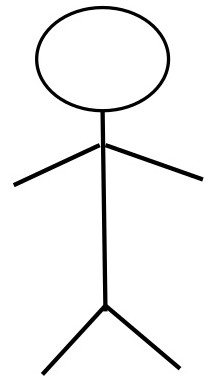
\includegraphics[height=0.02\textwidth]{Actor.jpg}
                            \label{Actor} El usuario ingresa al sistema por medio de la URL correspondiente
                            \item 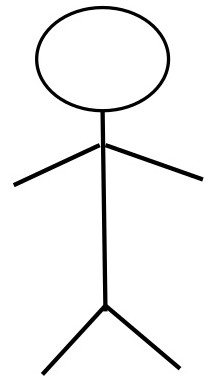
\includegraphics[height=0.02\textwidth]{Actor.jpg}
                            \label{Actor} El usuario visualizará la pantalla \ref{P2 Iniciar Sesión} podrá seleccionar la opción para poder ingresar al sistema si cuenta con una cuenta y deberá introducir las credenciales necesarias para poder ingresar al sistema en caso de contar con ellas.
                            \item 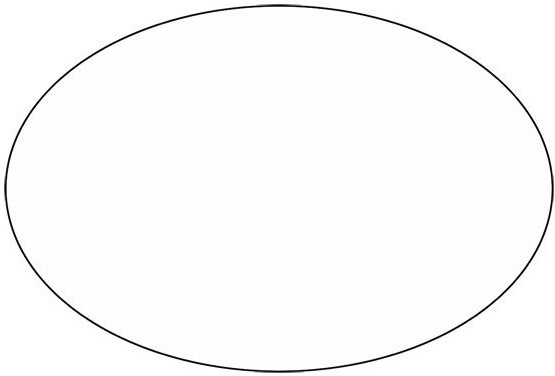
\includegraphics[height=0.02\textwidth]{Sistema.jpg}
                            \label{Sistema} El sistema comprobará que los campos ingresados por el actor existan en la base de datos y sean correctos. \ref{BR1 Acceso al sistema}
                            \item 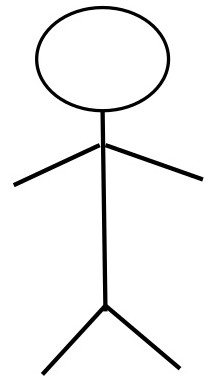
\includegraphics[height=0.02\textwidth]{Actor.jpg}
                            \label{Actor} El actor accede exitosamente y el sistema lo redirige a la pantalla \ref{P3 Vista Principal}
.
                        \end{enumerate}
                        
                        \vspace{0.3cm}\textbf{-- Fin del caso de uso}
                    \end{quote}
                
                    \vspace{0.5cm}\textbf{Trayectoria Alternativa A}\label{CU-1.0 Trayectoria Alternativa A}
                    \begin{quote}
                        \item A-1 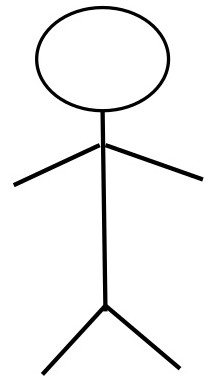
\includegraphics[height=0.02\textwidth]{Actor.jpg}
                            \label{Actor} El usuario ingresará el sistema por medio de la URL correspondiente. En caso de ser un usuario nuevo deberá ingresar los datos correspondientes para registrarse. \ref{P1 Crear Cuenta}
                        \item A-2 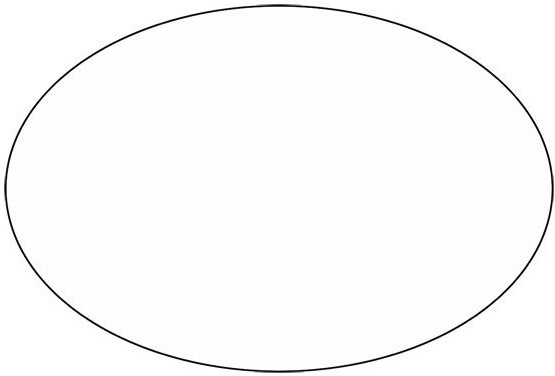
\includegraphics[height=0.02\textwidth]{Sistema.jpg}
                            \label{Sistema} El sistema validará los datos y en caso de que el usuario sea autorizado se creará la cuenta. \ref{BR1 Acceso al sistema}
                        \item A-3 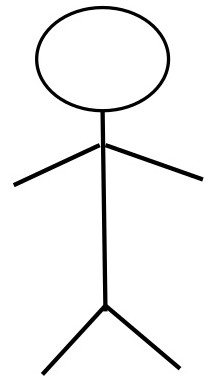
\includegraphics[height=0.02\textwidth]{Actor.jpg}
                            \label{Actor} El nuevo usuario contará con una cuenta para poder hacer uso de la trayectoria principal. \ref{CU-1.0 Trayectoria Principal}
                        
                        \vspace{0.3cm}\textbf{-- Fin del caso de uso}
                    \end{quote}
                
                    \vspace{0.5cm}\textbf{Trayectoria Alternativa B}\label{CU-1.0 Trayectoria Alternativa B}
                    \begin{quote}
                        \item B-1 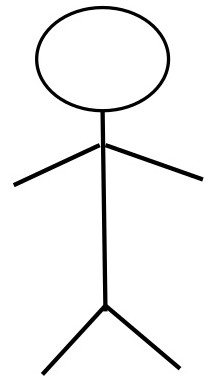
\includegraphics[height=0.02\textwidth]{Actor.jpg}
                            \label{Actor}  El usuario da click en el botón ingresar \ref{P2 Iniciar Sesión}
                        
\includegraphics[height=0.02\textwidth]{BotonIngresar.png}
                        \label{BotonIngresar}
                        \item B-2 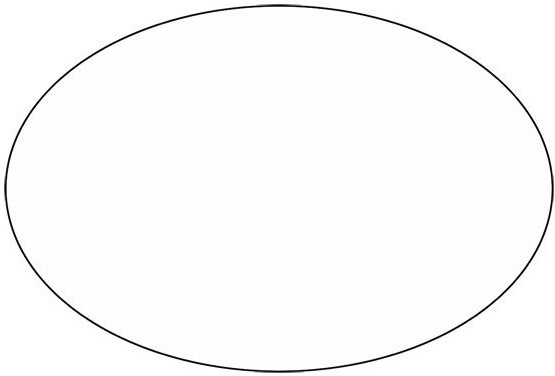
\includegraphics[height=0.02\textwidth]{Sistema.jpg}
                            \label{Sistema} El sistema comprobará que los datos ingresados por el actor son correctos. \ref{BR1 Acceso al sistema}
                        \item B-3 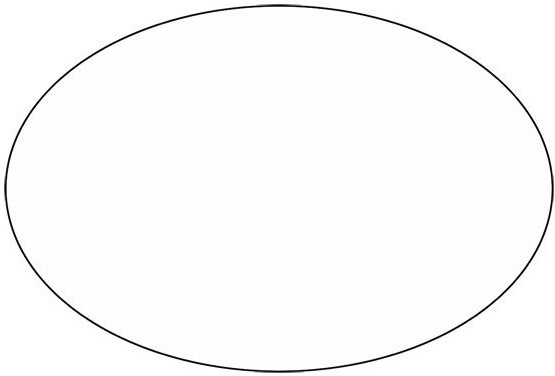
\includegraphics[height=0.02\textwidth]{Sistema.jpg}
                            \label{Sistema} El sistema encuentra que los datos son erróneos y muestra el mensaje de datos inválidos. 
                        \item B-4 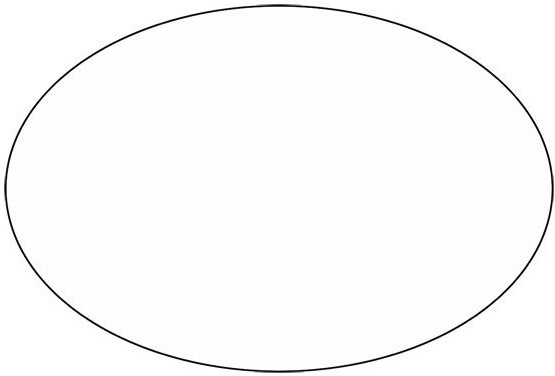
\includegraphics[height=0.02\textwidth]{Sistema.jpg}
                            \label{Sistema} El sistema redirige al usuario a la página principal. \ref{CU-1.0 Trayectoria Principal}
                        
                        \vspace{0.3cm}\textbf{-- Fin del caso de uso}
                    \end{quote}
                \end{quote}
        
            \newpage 
            \subsubsection{RIB-CU 1.1 Ingresar a la página} \label{RIB-CU 1.1 Ingresar a la página}
                \begin{table}[H]
                    \begin{center}
                        \begin{tabular}{| l | l | }
                        \hline
                        Caso de Uso & RIB-CU 1.1 Ingresar a la página \\ \hline                    
                        Versión & 0.1  \\ \hline
                        \multicolumn{2}{ |c| }{Resumen de atributos} \\ \hline
                        Hereda de & Ninguno  \\\hline
                        Actor & - Administrador  \\
                            & - Vendedor  \\
                            & - Comprador  \\
                            & -Usuario Anónimo  \\ \hline
                        Propósito & Ingresar a la página para buscar productos en venta \\ \hline
                        Entradas & Ninguna \\ \hline                    
                        Salidas &  Pantalla inicial \\\hline
                        Reglas de negocio & Ninguna  \\\hline
                        Precondiciones & Ninguna  \\\hline
                        Postcondiciones & Ninguna \\\hline
                        Errores & - E1: Mantenimiento de la página  \\
                                & - E2: conexión inestable  \\
                                & - E3: Incompatibilidad del navegador  \\ \hline
                        Tipo & Primario \\\hline
                        Observaciones & Verificar la versión del navegador forzosamente  \\\hline
                        \end{tabular}
                    \caption{Caso de Uso 2}
                    \label{sec:caso de uso 2}
                    \end{center}
                \end{table}
        
                \textbf{Trayectorias del Caso de Uso}
                \vspace{0.5cm}\textbf{Trayectoria Principal}\label{CU-1.1 Trayectoria Principal}
                    \begin{quote}
                        \begin{enumerate}
                            \item 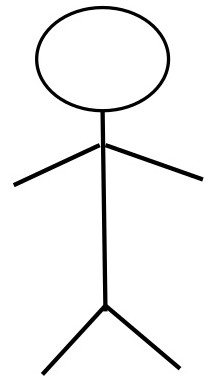
\includegraphics[height=0.02\textwidth]{Actor.jpg}
                            \label{Actor} El usuario ingresa por medio de la URL correspondiente \ref{CU-1.1 Trayectoria Alternativa A}\ref{CU-1.1 Trayectoria Alternativa B}\ref{CU-1.1 Trayectoria Alternativa C}
                            \item 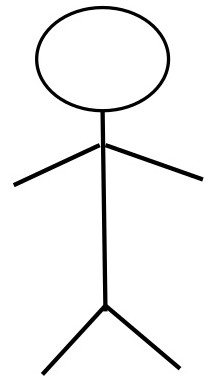
\includegraphics[height=0.02\textwidth]{Actor.jpg}
                            \label{Actor} El usuario accede a la pantalla inicial \ref{P3 Vista Principal}
                            \item 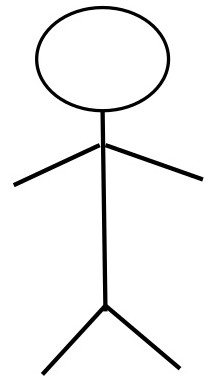
\includegraphics[height=0.02\textwidth]{Actor.jpg}
                            \label{Actor} El usuario puede realizar la búsqueda de productos en venta
                        
                            \vspace{0.3cm}\textbf{-- Fin del caso de uso}
                        \end{enumerate}
                    \end{quote}
                
                \vspace{0.5cm}\textbf{Trayectoria Alternativa A}\label{CU-1.1 Trayectoria Alternativa A}
                    \begin{quote}
                        \item A-1 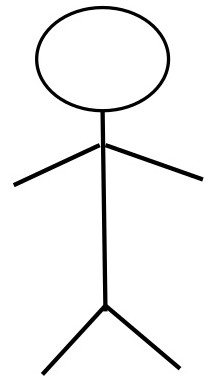
\includegraphics[height=0.02\textwidth]{Actor.jpg}
                            \label{Actor} El usuario ingresa la URL correspondiente mientras la pagina esta en mantenimiento \ref{PE Pantalla Error}
                        \item A-2 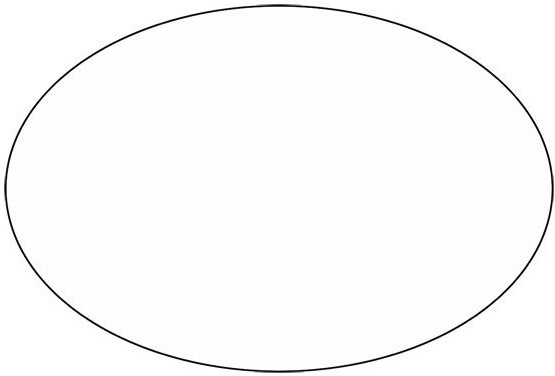
\includegraphics[height=0.02\textwidth]{Sistema.jpg}
                            \label{Sistema} El sistema muestra en pantalla el \ref{MSG1 Página en Mantenimiento} indicando al usuario que la página en ese momento no está disponible
                        \item A-3 Termina el caso de uso
                        
                        \vspace{0.3cm}\textbf{-- Fin del caso de uso}
                    \end{quote}
                
                \vspace{0.5cm}\textbf{Trayectoria Alternativa B}\label{CU-1.1 Trayectoria Alternativa B}
                    \begin{quote}
                        \item B-1 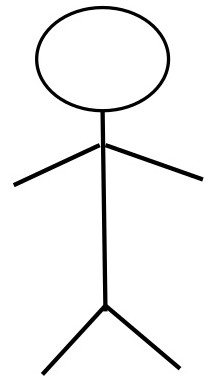
\includegraphics[height=0.02\textwidth]{Actor.jpg}
                            \label{Actor} El usuario ingresa la URL correspondiente desde una conexión inestable ref{PE Pantalla Error}
                        \item B-2 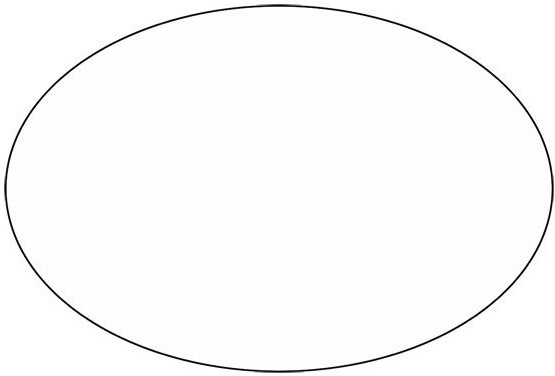
\includegraphics[height=0.02\textwidth]{Sistema.jpg}
                            \label{Sistema} El sistema muestra en pantalla el \ref{MSG2 Conexión Inestable} indicando al usuario que la página no funcionará de manera correcta
                        \item B-3 Termina caso de uso
                        
                        \vspace{0.3cm}\textbf{-- Fin del caso de uso}
                    \end{quote}
                
                \vspace{0.5cm}\textbf{Trayectoria Alternativa C}\label{CU-1.1 Trayectoria Alternativa C}
                    \begin{quote}
                        \item C-1 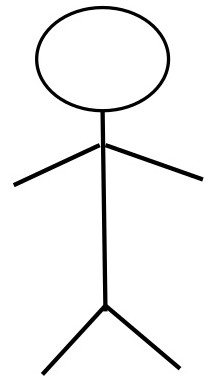
\includegraphics[height=0.02\textwidth]{Actor.jpg}
                            \label{Actor} El usuario ingresa la URL correspondiente desde un navegador incompatible \ref{PE Pantalla Error}
                        \item  C-2 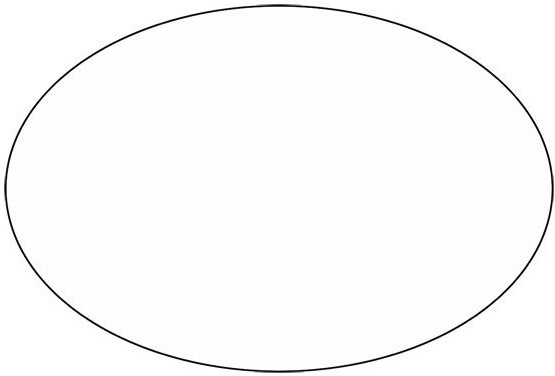
\includegraphics[height=0.02\textwidth]{Sistema.jpg}
                            \label{Sistema} El sistema muestra en pantalla el \ref{MSG3 Incompatibilidad del Navegador} indicando al usuario que no se puede acceder a la página
                        \item C-3 Termina caso de uso
                        
                        \vspace{0.3cm}\textbf{-- Fin del caso de uso}
                    \end{quote}
            
            \newpage 
            \subsubsection{RIB-CU 1.2 Buscar Productos}\label{RIB-CU 1.2 Buscar Productos}
                \begin{table}[H]
                    \begin{center}
                        \begin{tabular}{| l | l | }
                        \hline
                        Caso de Uso & RIB-CU 1.2 Buscar productos \\ \hline                    
                        Versión & 0.1  \\ \hline
                        \multicolumn{2}{ |c| }{Resumen de atributos} \\ \hline
                        Hereda de & Ninguno  \\\hline
                        Actor & - Administrador  \\
                            & - Vendedor  \\
                            & - Comprador  \\
                            & -Usuario Anónimo  \\ \hline
                        Propósito & Encontrar el producto deseado o requerido, comparar precios y productos similares \\ \hline
                        Entradas & El usuario ingresara el nombre o marca del producto \\
                                & El usuario podrá utilizar la función de filtrar por categorías, rango de precio\\ \hline
                        Salidas &  - Lista de categorías \\
                                &  - Lista de productos \\\hline
                        Reglas de negocio & BR12 Control de stock  \\\hline
                        Precondiciones & Ingresar a la página web  \\\hline
                        Postcondiciones & Ninguna \\\hline
                        Errores & - E1: Mantenimiento de la página  \\
                                & - E2: Sin resultado  \\
                                & - E3: Incompatibilidad del navegador  \\ \hline
                        Tipo & Primario \\\hline
                        Observaciones & Ninguna  \\\hline
                        \end{tabular}
                    \caption{Caso de Uso 3}
                    \label{sec:caso de uso 3}
                    \end{center}
                \end{table}
        
                \textbf{Trayectorias del Caso de Uso}
                \vspace{0.5cm}\textbf{Trayectoria Principal}\label{CU-1.2 Trayectoria Principal}
                    \begin{quote}
                        \begin{enumerate}
                            \item 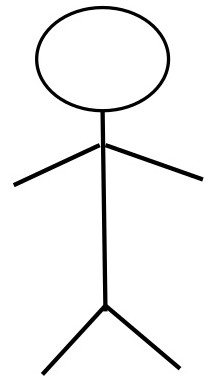
\includegraphics[height=0.02\textwidth]{Actor.jpg}
                            \label{Actor} El usuario inicia sesión y visualiza \ref{P3 Vista Principal}
                            \item 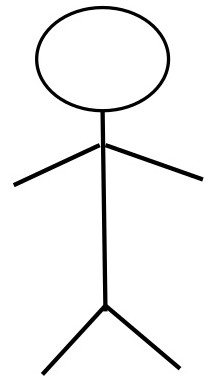
\includegraphics[height=0.02\textwidth]{Actor.jpg}
                            \label{Actor} El usuario dará clic a la barra de búsqueda de productos 
                            
\includegraphics[height=0.02\textwidth]{BarraDeBusqueda.jpg}
                            \label{BarraDeBusqueda}
                            \item 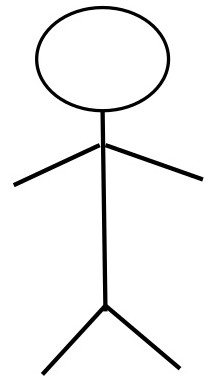
\includegraphics[height=0.02\textwidth]{Actor.jpg}
                            \label{Actor} El usuario ingresa el nombre del producto deseado
                            \item 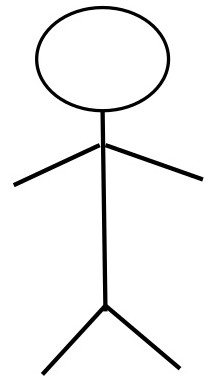
\includegraphics[height=0.02\textwidth]{Actor.jpg}
                            \label{Actor} El usuario da click al botón de Buscar u oprime la tecla Enter. \ref{P4 Búsqueda de Producto}
                            
\includegraphics[height=0.02\textwidth]{BotonBuscar.jpg}
                            \label{BotonBuscar}
                            \item 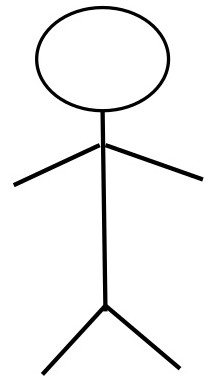
\includegraphics[height=0.02\textwidth]{Actor.jpg}
                            \label{Actor} El usuario podría dar click al botón Categorías \ref{CU-1.2 Trayectoria Alternativa A}
                            
\includegraphics[height=0.02\textwidth]{BotonCategorias.jpg}
                            \label{BotonCategorias}
                            \item 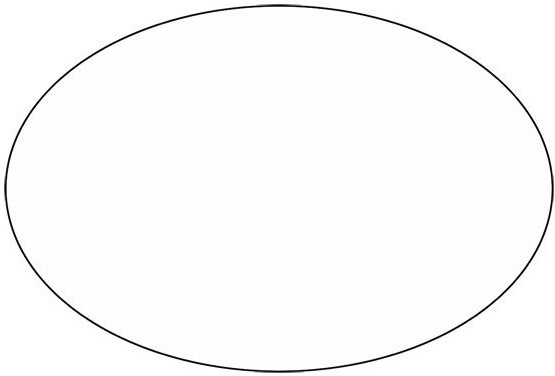
\includegraphics[height=0.02\textwidth]{Sistema.jpg}
                            \label{Sistema} El sistema muestra en la pantalla \ref{P4 Búsqueda de Producto} la lista de productos que coincidan con el producto que el usuario ingreso \ref{CU-1.2 Trayectoria Alternativa B}

                        
                            \vspace{0.3cm}\textbf{-- Fin del caso de uso}
                        \end{enumerate}
                    \end{quote}
                        
                \vspace{0.5cm}\textbf{Trayectoria Alternativa A}\label{CU-1.2 Trayectoria Alternativa A}
                    \begin{quote}
                        \item A-1 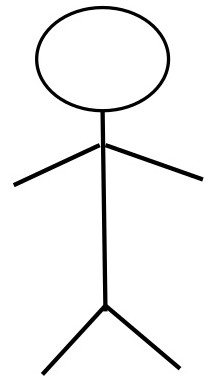
\includegraphics[height=0.02\textwidth]{Actor.jpg}
                            \label{Actor} El usuario oprime la sección de buscar productos por categoría \ref{P4 Búsqueda de Producto}
                        \item A-2 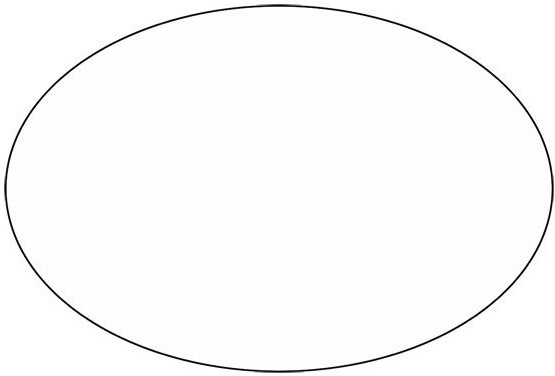
\includegraphics[height=0.02\textwidth]{Sistema.jpg}
                            \label{Sistema} El sistema le pide ingresar la categoría del producto a buscar
                        \item A-3 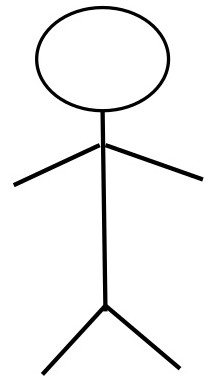
\includegraphics[height=0.02\textwidth]{Actor.jpg}
                            \label{Actor} El usuario ingresa la categoría \ref{CU-1.2 Trayectoria Alternativa B}
                        \item A-4 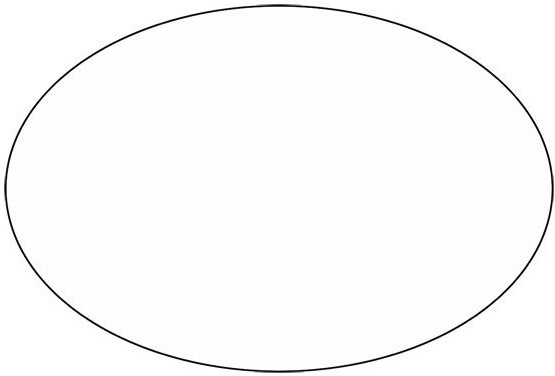
\includegraphics[height=0.02\textwidth]{Sistema.jpg}
                            \label{Sistema} El sistema muestra en pantalla la lista de categorías que coincidan con lo ingresado por el usuario \ref{P4 Búsqueda de Producto}
                        
                        \vspace{0.3cm}\textbf{-- Fin del caso de uso}
                    \end{quote}
                
                \vspace{0.5cm}\textbf{Trayectoria Alternativa B}\label{CU-1.2 Trayectoria Alternativa B}
                    \begin{quote}
                        \item B-1 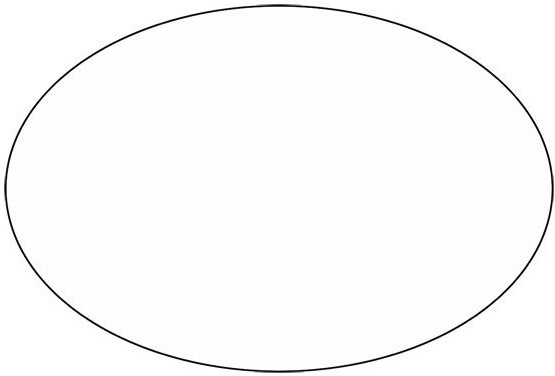
\includegraphics[height=0.02\textwidth]{Sistema.jpg}
                            \label{Sistema} El sistema no encuentra ningún resultado que coincida con la búsqueda del usuario \ref{PE Pantalla Error}
                        \item B-2 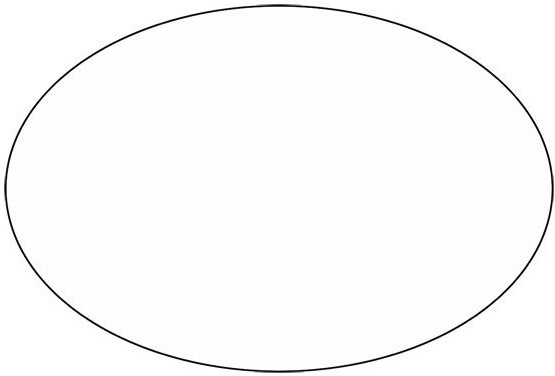
\includegraphics[height=0.02\textwidth]{Sistema.jpg}
                            \label{Sistema} El sistema muestra en pantalla el \ref{MSG4 Sin Resultados} indicando al usuario que no se encontró el producto solicitado
                        
                        \vspace{0.3cm}\textbf{-- Fin del caso de uso}
                    \end{quote}
                 
            \newpage 
            \subsubsection{RIB-CU 1.3 Ver Detalle de Producto}
                \begin{table}[H]
                    \begin{center}
                        \begin{tabular}{| l | l | }
                        \hline
                        Caso de Uso & RIB-CU 1.3 Ver detalle de producto. \\ \hline
                        
                        Versión & 0.1  \\ \hline
                        \multicolumn{2}{ |c| }{Resumen de atributos} \\ \hline
                        Hereda de & Buscar producto  \\\hline
                        Actor & - Administrador  \\
                            & - Vendedor  \\
                            & - Comprador  \\
                            & -Usuario Anónimo  \\ \hline
                        Propósito & Visualizar la información como las características, precio y vendedor  \\ \hline
                        Entradas & Ninguna \\ \hline
                        Salidas &  - Características del producto \\
                                &  - Precio del producto \\
                                &  - Datos del vendedor \\
                                &  - Imágenes del producto \\ \hline
                        Reglas de negocio & - BR10 Preguntas y Respuestas \\
                                        & - BR12 Control de stock \\\hline
                        Precondiciones & - Ingresar a la página web \\
                                    & - El usuario debe haber seleccionado un producto\\\hline
                        Postcondiciones & Ninguna \\\hline
                        Errores & - E1: Mantenimiento de la página  \\
                                & - E2: Recursos no encontrados  \\
                                & - E3: Incompatibilidad del navegador  \\ \hline
                        Tipo & Primario \\\hline
                        Observaciones & Ninguna  \\\hline
                        \end{tabular}
                    \caption{Caso de Uso 3}
                    \label{sec:caso de uso 3}
                    \end{center}
                \end{table}
                
                \textbf{Trayectorias del Caso de Uso}
                \vspace{0.5cm}\textbf{Trayectoria Principal}\label{CU-1.3 Trayectoria Principal}
                    \begin{quote}
                        \begin{enumerate}
                            \item  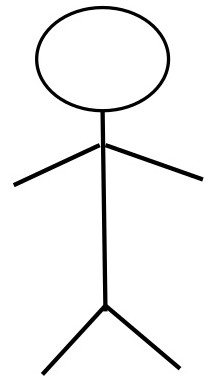
\includegraphics[height=0.02\textwidth]{Actor.jpg}
                            \label{Actor} El usuario realiza una búsqueda de productos \ref{P4 Búsqueda de Producto} y selecciona uno. 
                            \item  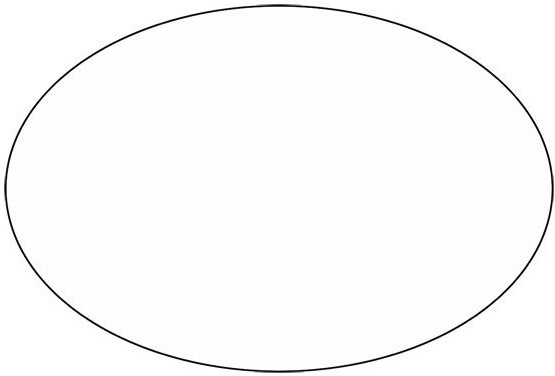
\includegraphics[height=0.02\textwidth]{Sistema.jpg}
                            \label{Sistema} En la pantalla \ref{P5 Descripción de un Producto} el usuario visualiza los detalles del producto \ref{CU-1.3 Trayectoria Alternativa A}
                            \item  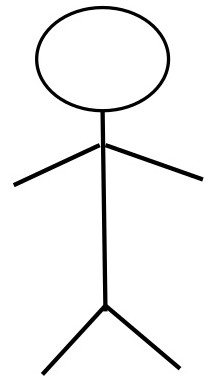
\includegraphics[height=0.02\textwidth]{Actor.jpg}
                            \label{Actor} El usuario selecciona comprar ahora
                            
\includegraphics[height=0.02\textwidth]{BotonComprarAhora.jpg}
                            \label{BotonComprarAhora}
                            \item  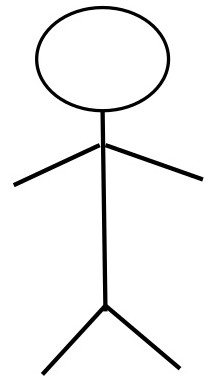
\includegraphics[height=0.02\textwidth]{Actor.jpg}
                            \label{Actor} El usuario puede agregar el producto al carrito \ref{CU-1.3 Trayectoria Alternativa D}
                        
                            \vspace{0.3cm}\textbf{-- Fin del caso de uso}
                        \end{enumerate}
                    \end{quote}
                        
                \vspace{0.5cm}\textbf{Trayectoria Alternativa A}\label{CU-1.3 Trayectoria Alternativa A}
                    \begin{quote}
                        \item A-1  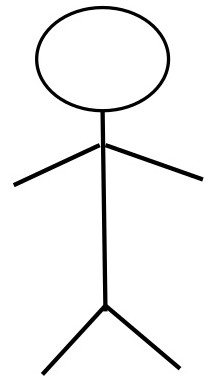
\includegraphics[height=0.02\textwidth]{Actor.jpg}
                            \label{Actor} El usuario hace una pregunta al vendedor \ref{CU-1.3 Trayectoria Alternativa B}
                        \item A-2 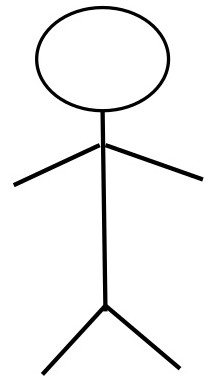
\includegraphics[height=0.02\textwidth]{Actor.jpg}
                            \label{Actor} El vendedor contesta
                        \item A-3  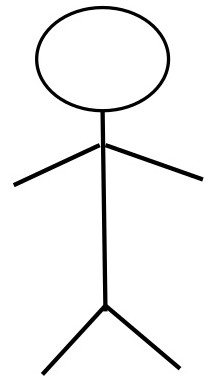
\includegraphics[height=0.02\textwidth]{Actor.jpg}
                            \label{Actor} El usuario puede agregar al carrito \ref{CU-1.3 Trayectoria Alternativa D}
                        
                        \vspace{0.3cm}\textbf{-- Fin del caso de uso}
                    \end{quote}
                
                \vspace{0.5cm}\textbf{Trayectoria Alternativa B}\label{CU-1.3 Trayectoria Alternativa B}
                    \begin{quote}
                        \item B-1  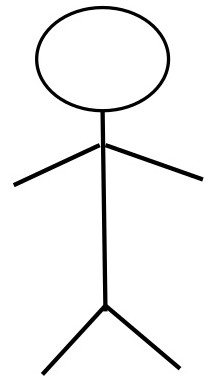
\includegraphics[height=0.02\textwidth]{Actor.jpg}
                            \label{Actor} El vendedor no contesta
                        \item B-2  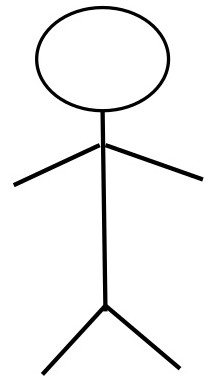
\includegraphics[height=0.02\textwidth]{Actor.jpg}
                            \label{Actor} El usuario no agrega el producto al carrito
                        
                        \vspace{0.3cm}\textbf{-- Fin del caso de uso}
                    \end{quote}
                
                \vspace{0.5cm}\textbf{Trayectoria Alternativa C}\label{CU-1.3 Trayectoria Alternativa C}
                    \begin{quote}
                        \item C-1  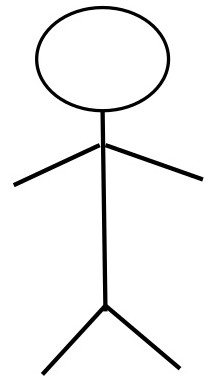
\includegraphics[height=0.02\textwidth]{Actor.jpg}
                            \label{Actor} El usuario ignora los detalles y va directo agregarlo al carrito \ref{CU-1.3 Trayectoria Alternativa D}
                        
                        \vspace{0.3cm}\textbf{-- Fin del caso de uso}
                    \end{quote}
                
                \vspace{0.5cm}\textbf{Trayectoria Alternativa D}\label{CU-1.3 Trayectoria Alternativa D}
                    \begin{quote}
                        \item D-1  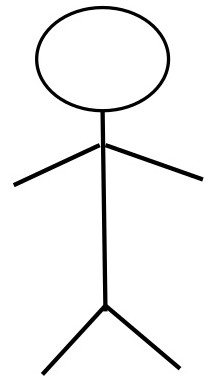
\includegraphics[height=0.02\textwidth]{Actor.jpg}
                            \label{Actor} El usuario selecciona cantidad y características del producto
                        \item D-2  \includegraphics[height=0.02\textwidth]{Actor.jpg}
                            \label{Actor} El usuario da click al botón “Agregar al carrito” \ref{MSG5 Producto Agregado con Éxito}
                        \includegraphics[height=0.02\textwidth]{BotonAgregarAlCarrito.jpg}
                        \label{BotonAgregarAlCarrito}
                        
                        \vspace{0.3cm}\textbf{-- Fin del caso de uso}
                    \end{quote}
                     
            \newpage 
            \subsubsubsection{RIB-CU 1.5 Gestionar carrito}\label{RIB-CU 1.5 Gestionar carrito}
                \begin{table}[H]
                    \begin{center}
                        \begin{tabular}{| l | l | }
                        \hline
                        Caso de Uso & RIB-CU 1.5 Gestionar carrito \\ \hline
                        
                        Versión & 0.1  \\ \hline
                        \multicolumn{2}{ |c| }{Resumen de atributos} \\ \hline
                        Hereda de & - Eliminar producto \\
    		            	& - Visualizar producto \\\hline
                        Actor & - Administrador \\
                            & - Vendedor  \\
                            & - Comprador  \\
                            & -Usuario Anónimo \\ \hline
                        Propósito & Visualizar o eliminar los productos agregados al carrito \\ \hline
                        Entradas & Ninguna \\ \hline
                        Salidas & - El usuario podrá visualizar el nombre, imagen del producto y dos botones, uno para\\ & eliminarlo y otro para ir a los detalles del producto \\
                    			& - El producto eliminado no se mostrará \\
    			                & - Proceder al método de pago \\
    			                & - Continuar con el proceso de compra \\ \hline
                        Reglas de negocio & BR12 Control de stock \\\hline
                        Precondiciones & - El usuario tendrá que haber agregado por lo menos un producto al carrito \\ \hline
                        Postcondiciones & El sistema actualizará el carrito en caso de eliminar un producto \\\hline
                        Errores & - E1: Imposible eliminar el producto  \\
                                & - E2: Imposible visualizar el producto  \\ \hline
                        Tipo & Primario \\\hline
                        Observaciones & Ninguna  \\\hline
                        \end{tabular}
                    \caption{Caso de Uso 5}
                    \label{sec:caso de uso 5}
                    \end{center}
                \end{table}
        
                \textbf{Trayectorias del Caso de Uso}
                \vspace{0.5cm}\textbf{Trayectoria Principal}\label{CU-1.5 Trayectoria Principal}
                    \begin{quote}
                        \begin{enumerate}
                            \item  \includegraphics[height=0.02\textwidth]{Actor.jpg}
                            \label{Actor} El usuario da click en el botón agregar al carrito y visualiza la pantalla \ref{P10 Carrito de Compra}
                            \item  \includegraphics[height=0.02\textwidth]{Actor.jpg}
                            \label{Actor} El usuario visualiza la pantalla de Carrito de compra
                            \item  \includegraphics[height=0.02\textwidth]{Actor.jpg}
                            \label{Actor} El usuario puede dar click en el botón Agregar al carrito \ref{CU-1.5 Trayectoria Alternativa A}
                            \includegraphics[height=0.02\textwidth]{BotonAgregarAlCarrito.jpg}
                            \label{BotonAgregarAlCarrito}
                            \item  \includegraphics[height=0.02\textwidth]{Actor.jpg}
                            \label{Actor} El usuario puede dar click en el botón Eliminar producto \ref{CU-1.5 Trayectoria Alternativa B}
                            \includegraphics[height=0.02\textwidth]{BotonEliminarProducto.png}
                            \label{BotonEliminarProducto}
                            \item  \includegraphics[height=0.02\textwidth]{Actor.jpg}
                            \label{Actor} El usuario puede dar click en el botón comprar ahora \ref{P6 Envío de Compra}
                            \includegraphics[height=0.02\textwidth]{BotonComprarAhora.jpg}
                            \label{BotonComprarAhora}
                        
                            \vspace{0.3cm}\textbf{-- Fin del caso de uso}
                        \end{enumerate}
                    \end{quote}
                        
                \vspace{0.5cm}\textbf{Trayectoria Alternativa A}\label{CU-1.5 Trayectoria Alternativa A}
                    \begin{quote}
                        \item A-1  \includegraphics[height=0.02\textwidth]{Actor.jpg}
                            \label{Actor} El usuario modifica la cantidad o características de los productos \ref{MSG6 Producto Actualizado}
                        
                        \vspace{0.3cm}\textbf{-- Fin del caso de uso}
                    \end{quote}
                
                \vspace{0.5cm}\textbf{Trayectoria Alternativa B}\label{CU-1.5 Trayectoria Alternativa B}
                    \begin{quote}
                        \item B-1  \includegraphics[height=0.02\textwidth]{Actor.jpg}
                            \label{Actor} El usuario eliminará ciertos productos del carrito \ref{MSG7 Producto Eliminado}
                        
                        \vspace{0.3cm}\textbf{-- Fin del caso de uso}
                    \end{quote}
                   
            \newpage 
            \subsubsection{RIB-CU 1.6 Crear Cuenta}\label{RIB-CU 1.6 Iniciar Sesión}
                \begin{table}[H]
                    \begin{center}
                        \begin{tabular}{| l | l | }
                        \hline
                        Caso de Uso & RIB-CU 1.6 Crear Cuenta \\ \hline
                        
                        Versión & 0.1  \\ \hline
                        \multicolumn{2}{ |c| }{Resumen de atributos} \\ \hline
                        Hereda de & Ninguno \\\hline
                        Actor & Usuario anónimo \\ \hline
                        Propósito & Poder crear una cuenta nueva \\ \hline
                        Entradas & Correo institucional\\
                                & Nombre de usuario\\
                                & Contraseña \\ \hline
                        Salidas & Mensaje de confirmación \\ \hline
                        Reglas de negocio & BR1 Acceso al sistema \\\hline
                        Precondiciones & - Ingresar a la página \\
                                    & - No se tene una cuenta \\ \hline
                        Postcondiciones & El usuario tendrá una cuenta \\\hline
                        Errores & - E1: Formato de contraseña incorrecto \\
                                & - E2: Correo inválido \\ \hline
                        Tipo & Primario \\\hline
                        Observaciones & Ninguna  \\\hline
                        \end{tabular}
                    \caption{Caso de Uso 6}
                    \label{sec:caso de uso 6}
                    \end{center}
                \end{table}
        
                \textbf{Trayectorias del Caso de Uso}
                \vspace{0.5cm}\textbf{Trayectoria Principal}\label{CU-1.6 Trayectoria Principal}
                    \begin{quote}
                        \begin{enumerate}
                            \item  \includegraphics[height=0.02\textwidth]{Actor.jpg}
                            \label{Actor} El usuario da clic en crear cuenta y accede a través de la página \ref{P1 Crear Cuenta} 
                            \item  \includegraphics[height=0.02\textwidth]{Actor.jpg}
                            \label{Actor} El usuario ingresará los datos correspondientes
                            \item  \includegraphics[height=0.02\textwidth]{Sistema.jpg}
                            \label{Sistema} El sistema validará su cuenta \ref{BR1 Acceso al sistema}
                            \item  \includegraphics[height=0.02\textwidth]{Actor.jpg}
                            \label{Actor} El usuario dará clic en el botón 
                            \includegraphics[height=0.02\textwidth]{BotonCrearCuenta.jpg}
                            \label{BotonCrearCuenta} crear cuenta e ingresará a la pantalla de Iniciar Sesión \ref{P2 Iniciar Sesión}
                            \item  \includegraphics[height=0.02\textwidth]{Actor.jpg}
                            \label{Actor} El usuario puede tener datos incorrectos \ref{CU-1.5 Trayectoria Alternativa A} \ref{CU-1.6 Trayectoria Alternativa B}
                        
                            \vspace{0.3cm}\textbf{-- Fin del caso de uso}
                        \end{enumerate}
                    \end{quote}
                        
                \vspace{0.5cm}\textbf{Trayectoria Alternativa A}\label{CU-1.6 Trayectoria Alternativa A}
                    \begin{quote}
                        \item A-1  \includegraphics[height=0.02\textwidth]{Actor.jpg}
                            \label{Actor} El usuario ingreso un formato de contraseña incorrecto \ref{MSG9 Correo Inválido}
                        
                        \vspace{0.3cm}\textbf{-- Fin del caso de uso}
                    \end{quote}
                
                \vspace{0.5cm}\textbf{Trayectoria Alternativa B}\label{CU-1.6 Trayectoria Alternativa B}
                    \begin{quote}
                        \item B-1  \includegraphics[height=0.02\textwidth]{Actor.jpg}
                            \label{Actor} El usuario ingreso un formato de contraseña incorrecto \ref{MSG8 Formato de Contraseña Incorrecto}
                        
                        \vspace{0.3cm}\textbf{-- Fin del caso de uso}
                    \end{quote}
                
            \newpage 
            \subsubsection{RIB-CU 1.7 Gestionar método de pago}\label{RIB-CU 1.7 Gestionar método de pago}
                \begin{table}[H]
                    \begin{center}
                        \begin{tabular}{| l | l | }
                        \hline
                        Caso de Uso & RIB-CU 1.7 Gestionar método de pago \\ \hline
                        
                        Versión & 0.1  \\ \hline
                        \multicolumn{2}{ |c| }{Resumen de atributos} \\ \hline
                        Hereda de & Iniciar sesión \\\hline
                        Actor & - Usuario registrado \\ \hline
                        Propósito & Visualizar o eliminar los distintos métodos de pago \\ \hline
                        Entradas & Ninguna \\ \hline
                        Salidas &  El usuario podrá visualizar el listado de sus tarjetas\\
                                & Tres botones uno para agregar, otro para editar y otro para eliminar \\ \hline
                        Reglas de negocio & BR3: Validación bancaria \\\hline
                        Precondiciones & El usuario debe haber registrado por lo menos un método de pago \\\hline
                        Postcondiciones &El sistema deberá guardar los cambios realizados \\\hline
                        Errores & - E1: Información no encontrada  \\ \hline
                        Tipo & Primario \\\hline
                        Observaciones & Ninguna  \\\hline
                        \end{tabular}
                    \caption{Caso de Uso 7}
                    \label{sec:caso de uso 7}
                    \end{center}
                \end{table}
                
                \textbf{Trayectorias del Caso de Uso}
                \vspace{0.5cm}\textbf{Trayectoria Principal}\label{CU-1.7 Trayectoria Principal}
                    \begin{quote}
                        \begin{enumerate}
                            \item  \includegraphics[height=0.02\textwidth]{Actor.jpg}
                            \label{Actor}  El usuario da click en el botón Ir a métodos de pago y visualiza la pantalla \ref{P10 Carrito de Compra} 
                            \includegraphics[height=0.02\textwidth]{BotonGestionarMetodosDePago.png}
                            \label{BotonGestionarMetodosDePago}
                            \item  \includegraphics[height=0.02\textwidth]{Actor.jpg}
                            \label{Actor}  El usuario visualiza la pantalla \ref{P12 Direcciones de Envío}
                            \item  \includegraphics[height=0.02\textwidth]{Actor.jpg}
                            \label{Actor} El usuario puede dar click en el botón
                            \includegraphics[height=0.02\textwidth]{BotonAgregarMetodoDePago.jpg}
                            \label{BotonAgregarMetodoDePago}
                            Agregar método de pago \ref{CU-1.7 Trayectoria Alternativa A}
                            \item  \includegraphics[height=0.02\textwidth]{Actor.jpg}
                            \label{Actor} El usuario puede dar click en el botón Eliminar método de pago \ref{CU-1.7 Trayectoria Alternativa B} 
                            \includegraphics[height=0.02\textwidth]{BotonEliminarMetodosDePago.png}
                            \label{BotonEliminarMetodosDePago}
                            \vspace{0.3cm}
                            
                            \textbf{-- Fin del caso de uso}
                        \end{enumerate}
                    \end{quote}
                        
                \vspace{0.5cm}\textbf{Trayectoria Alternativa A}\label{CU-1.7 Trayectoria Alternativa A}
                    \begin{quote}
                        \item A-1   \includegraphics[height=0.02\textwidth]{Actor.jpg}
                            \label{Actor} El usuario modifica los datos del método de pago \ref{MSG10 Método Actualizado}
                        
                        \vspace{0.3cm}\textbf{-- Fin del caso de uso}
                    \end{quote}
                
                \vspace{0.5cm}\textbf{Trayectoria Alternativa B}\label{CU-1.7 Trayectoria Alternativa B}
                    \begin{quote}
                        \item B-1  \includegraphics[height=0.02\textwidth]{Actor.jpg}
                            \label{Actor} El usuario eliminará el método de pago \ref{MSG11 Método Eliminado}
                        
                        \vspace{0.3cm}\textbf{-- Fin del caso de uso}
                    \end{quote}
              
            \newpage        
            \subsubsection{RIB-CU 1.8 Registrar método de pago}\label{RIB-CU 1.8 Registrar método de pago}
                \begin{table}[H]
                    \begin{center}
                        \begin{tabular}{| l | l | }
                        \hline
                        Caso de Uso & RIB-CU 1.8 Registrar método de pago \\ \hline
                        
                        Versión & 0.1  \\ \hline
                        \multicolumn{2}{ |c| }{Resumen de atributos} \\ \hline
                        Hereda de & Gestionar método de pago \\\hline
                        Actor & Usuario registrado \\ \hline
                        Propósito & Añadir una forma de pago para realizar compras \\ \hline
                        Entradas & - El usuario ingresará los 16 dígitos de la tarjeta \\
                                & - El usuario ingresará la fecha de vencimiento de la tarjeta \\
                                & - El usuario ingresará el código de seguridad de la tarjeta \\ \hline
                        Salidas & Validación bancaria exitosa \\ \hline
                        Reglas de negocio & BR3: Validación bancaria \\\hline
                        Precondiciones & El usuario debe contar con una cuenta bancaria y un tarjeta ya sea de credito o debito \\ \hline
                        Postcondiciones & El usuario podrá realizar comprar a través de su método de pago \\\hline
                        Errores & - E1: Tarjeta invalida \\
                                & - E2: Tarjeta expirada \\
                                & - E3: Información bancaria incorrecta  \\ \hline
                        Tipo & Primario \\\hline
                        Observaciones & Ninguna  \\\hline
                        \end{tabular}
                    \caption{Caso de Uso 8}
                    \label{sec:caso de uso 8}
                    \end{center}
                \end{table}
        
                \textbf{Trayectorias del Caso de Uso}
                \vspace{0.5cm}\textbf{Trayectoria Principal}\label{CU-1.8 Trayectoria Principal}
                    \begin{quote}
                        \begin{enumerate}
                            \item  \includegraphics[height=0.02\textwidth]{Actor.jpg}
                            \label{Actor} El usuario da click en el botón agregar método de pago y visualiza la pantalla \ref{P12 Direcciones de Envío} 
                            \includegraphics[height=0.02\textwidth]{BotonAgregarMetodoDePago.jpg}
                            \label{BotonAgregarMetodoDePago}
                            \item  \includegraphics[height=0.02\textwidth]{Actor.jpg}
                            \label{Actor} El usuario ingresa y selecciona los datos requeridos
                            \item  \includegraphics[height=0.02\textwidth]{Actor.jpg}
                            \label{Actor} El usuario puede dar click en el botón “Agregar tarjeta” 
                            \includegraphics[height=0.02\textwidth]{BotonAgregarTarjeta.png}
                            \label{BotonAgregarrTarjeta}\ref{CU-1.8 Trayectoria Alternativa A}
                            \item  \includegraphics[height=0.02\textwidth]{Actor.jpg}
                            \label{Actor} El usuario puede dar click en el botón “Cerrar” 
                            \includegraphics[height=0.02\textwidth]{BotonCerrar.png}
                            \label{BotonCerrar}
                            \item  \includegraphics[height=0.02\textwidth]{Sistema.jpg}
                            \label{Sistema} El sistema redirige al usuario a la pantalla anterior
                        
                            \vspace{0.3cm}\textbf{-- Fin del caso de uso}
                        \end{enumerate}
                    \end{quote}
                        
                \vspace{0.5cm}\textbf{Trayectoria Alternativa A}\label{CU-1.8 Trayectoria Alternativa A}
                    \begin{quote}
                        \item A-1  \includegraphics[height=0.02\textwidth]{Sistema.jpg}
                            \label{Sistema} El sistema valida que los datos sean correctos y la tarjeta sea válida
                        \item A-2 Los datos pueden ser incorrectos \ref{CU-1.8 Trayectoria Alternativa B}
                        \item A-3  \includegraphics[height=0.02\textwidth]{Sistema.jpg}
                            \label{Sistema} El sistema encripta y guarda los datos de la tarjeta
                        \item A-4  \includegraphics[height=0.02\textwidth]{Sistema.jpg}
                            \label{Sistema}  El sistema muestra un mensaje de éxito \ref{MSG14 Tarjeta Registrada}
                        
                        \vspace{0.3cm}\textbf{-- Fin del caso de uso}
                    \end{quote}
                
                \vspace{0.5cm}\textbf{Trayectoria Alternativa B}\label{CU-1.8 Trayectoria Alternativa B}
                    \begin{quote}
                        \item B-1  \includegraphics[height=0.02\textwidth]{Sistema.jpg}
                            \label{Sistema} El sistema mostrará la pantalla de error \ref{PE Pantalla Error}
                        
                        \vspace{0.3cm}\textbf{-- Fin del caso de uso}
                    \end{quote}
                 
            \newpage    
            \subsubsection{RIB-CU 1.9 Registrar dirección de envío}\label{RIB-CU 1.9 Registrar dirección de envío}
                \begin{table}[H]
                    \begin{center}
                        \begin{tabular}{| l | l | }
                        \hline
                        Caso de Uso & RIB-CU 1.9 Registrar dirección de envío \\ \hline
                        
                        Versión & 0.1  \\ \hline
                        \multicolumn{2}{ |c| }{Resumen de atributos} \\ \hline
                        Hereda de & Ninguno \\\hline
                        Actor & Usuario registrado \\ \hline
                        Propósito & Añadir una dirección a donde puedan ser enviadas las órdenes hechas en la plataforma \\ \hline
                        Entradas & El usuario deberá proporcionar su calle, colonia, delegación, ciudad \\ \hline
                        Salidas & Validación de dirección exitosa \\ \hline
                        Reglas de negocio & BR13  Validación de dirección \\\hline
                        Precondiciones & Iniciar sesión. \\ \hline
                        Postcondiciones & El usuario podrá enviar sus órdenes a su dirección agregada \\\hline
                        Errores & - E1: Dirección invalida \\
                                & - E2: Fuera de la zona de cobertura  \\ \hline
                        Tipo & Primario \\\hline
                        Observaciones & Ninguna  \\\hline
                        \end{tabular}
                    \caption{Caso de Uso 9}
                    \label{sec:caso de uso 9}
                    \end{center}
                \end{table}
        
                \textbf{Trayectorias del Caso de Uso}
                \vspace{0.5cm}\textbf{Trayectoria Principal}\label{CU-1.9 Trayectoria Principal}
                    \begin{quote}
                        \begin{enumerate}
                            \item  \includegraphics[height=0.02\textwidth]{Actor.jpg}
                            \label{Actor} El usuario da click en el botón agregar método de entrega y visualiza la pantalla \ref{P6 Envío de Compra}
                            \includegraphics[height=0.02\textwidth]{BotonAgregarMetodoDeEntrega.jpg}
                            \label{BotonAgregarMetodoDeEntrega}
                            \item  \includegraphics[height=0.02\textwidth]{Actor.jpg}
                            \label{Actor} El usuario ingresa los datos requeridos
                            \item  \includegraphics[height=0.02\textwidth]{Actor.jpg}
                            \label{Actor} El usuario puede dar click en el botón “Agregar dirección” \includegraphics[height=0.02\textwidth]{BotonAgregarDireccion.png}
                            \label{BotonAgregarDireccion}
                            \item  \includegraphics[height=0.02\textwidth]{Actor.jpg}
                            \label{Actor} El usuario puede dar click en el botón “Cerrar” \includegraphics[height=0.02\textwidth]{BotonCerrar.png}
                            \label{BotonCerrar}
                            \item  \includegraphics[height=0.02\textwidth]{Sistema.jpg}
                            \label{Sistema} El sistema redirige al usuario a la pantalla anterior
                        
                        \vspace{0.3cm}\textbf{-- Fin del caso de uso}
                        \end{enumerate}
                    \end{quote}
                        
                \vspace{0.5cm}\textbf{Trayectoria Alternativa A}\label{CU-1.9 Trayectoria Alternativa A}
                    \begin{quote}
                        \item A-1  \includegraphics[height=0.02\textwidth]{Sistema.jpg}
                            \label{Sistema} El sistema valida que los datos sean correctos y la dirección sea válida
                        \item A-2 Los datos pueden ser incorrectos \ref{CU-1.9 Trayectoria Alternativa B}
                        \item A-3  \includegraphics[height=0.02\textwidth]{Sistema.jpg}
                            \label{Sistema} El sistema guarda la dirección
                        \item A-4  \includegraphics[height=0.02\textwidth]{Sistema.jpg}
                            \label{Sistema} El sistema muestra un mensaje de éxito \ref{MSG15 Dirección Registrada}
                        
                        \vspace{0.3cm}\textbf{-- Fin del caso de uso}
                    \end{quote}
                
                \vspace{0.5cm}\textbf{Trayectoria Alternativa B}\label{CU-1.9 Trayectoria Alternativa B}
                    \begin{quote}
                        \item B-1  \includegraphics[height=0.02\textwidth]{Sistema.jpg}
                            \label{Sistema} El sistema mostrará la pantalla de error \ref{PE Pantalla Error}
                        
                        \vspace{0.3cm}\textbf{-- Fin del caso de uso}
                    \end{quote}
                    
            \newpage 
            \subsubsection{RIB-CU 1.10 Gestionar Direcciones de Envío}\label{RIB-CU 1.10 Gestionar Direcciones de Envío}
                \begin{table}[H]
                    \begin{center}
                        \begin{tabular}{| l | l | }
                        \hline
                        Caso de Uso & RIB-CU 1.10 Gestionar Direcciones de Envío \\ \hline
                        
                        Versión & 0.1  \\ \hline
                        \multicolumn{2}{ |c| }{Resumen de atributos} \\ \hline
                        Hereda de & Ninguno \\\hline
                        Actor & Usuario registrado \\ \hline
                        Propósito & Visualizar, eliminar o modificar las direcciones de envío registradas \\ \hline
                        Entradas & - Ninguna \\ \hline
                        Salidas & El usuario podrá visualizar su dirección registrada \\
                                & Tres botones uno para visualizar, uno para editar y uno para eliminar \\ \hline
                        Reglas de negocio & Ninguna \\\hline
                        Precondiciones & El usuario debe haber registrado por lo menos una dirección de envío \\ \hline
                        Postcondiciones & El sistema debe almacenar, eliminar o actualizar los datos ingresados \\\hline
                        Errores & - E1: Información no encontrada  \\ \hline
                        Tipo & Primario \\\hline
                        Observaciones & Ninguna  \\\hline
                        \end{tabular}
                    \caption{Caso de Uso 10}
                    \label{sec:caso de uso 10}
                    \end{center}
                \end{table}
        
                \textbf{Trayectorias del Caso de Uso}
                \vspace{0.5cm}\textbf{Trayectoria Principal}\label{CU-1.10 Trayectoria Principal}
                    \begin{quote}
                        \begin{enumerate}
                            \item  \includegraphics[height=0.02\textwidth]{Actor.jpg}
                            \label{Actor} El usuario da click en el botón Ir a direcciones de envío y visualiza la pantalla \ref{P11 Métodos de Pago} \includegraphics[height=0.02\textwidth]{BotonDireccionDeEnvio.png}
                            \label{BotonDireccionDeEnvio}
                            \item A-2  \includegraphics[height=0.02\textwidth]{Actor.jpg}
                            \label{Actor} El usuario puede dar click en el botón Agregar dirección de envío \ref{CU-1.10 Trayectoria Alternativa A} \includegraphics[height=0.02\textwidth]{BotonAgregarDireccionDeEnvio.png}
                            \label{BotonAgregarDireccionDeEnvio}
                            \item A-3  \includegraphics[height=0.02\textwidth]{Actor.jpg}
                            \label{Actor} El usuario puede dar click en el botón Eliminar dirección de envío \ref{CU-1.10 Trayectoria Alternativa B} \includegraphics[height=0.02\textwidth]{BotonEliminarDireccion.png}
                            \label{BotonEliminarDireccion}
                            
                            \vspace{0.3cm}\textbf{-- Fin del caso de uso}
                        \end{enumerate}
                    \end{quote}
                
                \vspace{0.5cm}\textbf{Trayectoria Alternativa A}\label{CU-1.10 Trayectoria Alternativa A}
                    \begin{quote}
                        \item A-1  \includegraphics[height=0.02\textwidth]{Actor.jpg}
                            \label{Actor} El usuario modifica los datos dirección de envío \ref{MSG12 Dirección Actualizada}
                        
                        \vspace{0.3cm}\textbf{-- Fin del caso de uso}
                    \end{quote}
                   
                \vspace{0.5cm}\textbf{Trayectoria Alternativa B}\label{CU-1.10 Trayectoria Alternativa B}
                    \begin{quote}
                        \item B-1  \includegraphics[height=0.02\textwidth]{Actor.jpg}
                            \label{Actor} El usuario eliminará la dirección de envío \ref{MSG13 Dirección Eliminada}
                        
                        \vspace{0.3cm}\textbf{-- Fin del caso de uso}
                    \end{quote}
                
            \newpage    
            \subsubsection{RIB-CU 1.11 Confirmar compra}\label{RIB-CU 1.11 Confirmar compra}
                \begin{table}[H]
                    \begin{center}
                        \begin{tabular}{| l | l | }
                        \hline
                        Caso de Uso & RIB-CU 1.11 Confirmar compra \\ \hline
                        
                        Versión & 0.1  \\ \hline
                        \multicolumn{2}{ |c| }{Resumen de atributos} \\ \hline
                        Hereda de & Ninguno \\\hline
                        Actor & Usuario registrado \\ \hline
                        Propósito & Generar una orden con los productos agregados al carrito, enviarla a la dirección\\ & de envío seleccionada y pagar con el método de pago registrado \\ \hline
                        Entradas & El usuario deberá seleccionar el tipo de envío \\ \hline
                        Salidas & Número de pedido y fecha aproximada de entrega \\ \hline
                        Reglas de negocio & BR8: Método de envío \\
                                        & BR6 Control de ventas \\
                                        & BR4  Control de stock \\
                                        & BR2 Gestión de compras \\ \hline
                        Precondiciones & Haber generado un carrito, agregado un método de pago, agregado una \\ & dirección de envío \\ \hline
                        Postcondiciones & El pedido generado se mostrará en el apartado de las pedidos creados \\\hline
                        Errores & - E1: Pago no procesado  \\ \hline
                        Tipo & Primario \\\hline
                        Observaciones & Ninguna  \\\hline
                        \end{tabular}
                    \caption{Caso de Uso 11}
                    \label{sec:caso de uso 11}
                    \end{center}
                \end{table}
        
                \textbf{Trayectorias del Caso de Uso}
                \vspace{0.5cm}\textbf{Trayectoria Principal}\label{CU-1.11 Trayectoria Principal}
                    \begin{quote}
                        \begin{enumerate}
                            \item  \includegraphics[height=0.02\textwidth]{Actor.jpg}
                            \label{Actor} El usuario confirmará el caso de uso \ref{RIB-CU 1.7 Gestionar método de pago} o \ref{RIB-CU 1.8 Registrar método de pago}
                            \item  \includegraphics[height=0.02\textwidth]{Actor.jpg}
                            \label{Actor} El usuario confirmará el caso de uso \ref{RIB-CU 1.9 Registrar dirección de envío} o \ref{RIB-CU 1.10 Gestionar Direcciones de Envío}
                            \item  \includegraphics[height=0.02\textwidth]{Actor.jpg}
                            \label{Actor} El usuario dará clic en “Confirmar compra” \ref{CU-1.11 Trayectoria Alternativa A} \ref{CU-1.11 Trayectoria Alternativa B}
                        
                            \vspace{0.3cm}\textbf{-- Fin del caso de uso}
                        \end{enumerate}
                    \end{quote}
                        
                \vspace{0.5cm}\textbf{Trayectoria Alternativa A}\label{CU-1.11 Trayectoria Alternativa A}
                    \begin{quote}
                        \begin{enumerate}
                            \item  \includegraphics[height=0.02\textwidth]{Sistema.jpg}
                            \label{Sistema} El banco realiza el cargo correctamente y transfiere el pago al vendedor \ref{MSG16 Compra Exitosa}
                        
                        \vspace{0.3cm}\textbf{-- Fin del caso de uso}
                        \end{enumerate}
                    \end{quote}
                        
                \vspace{0.5cm}\textbf{Trayectoria Alternativa B}\label{CU-1.11 Trayectoria Alternativa B}
                    \begin{quote}
                        \begin{enumerate} \includegraphics[height=0.02\textwidth]{Sistema.jpg}
                            \label{Sistema} El banco no puede realizar el cargo \ref{MSG17 Compra Rechazada}
                        
                        \vspace{0.3cm}\textbf{-- Fin del caso de uso}
                        \end{enumerate}
                    \end{quote}
        \newpage
        \subsection{Diagramas de Casos de Uso}
            \vspace{1cm}
            \subsubsection{CU-A Administrador}\
            \vspace{1cm}
            \includegraphics[height=0.65\textwidth]{CasoDeUsoAdministrador.jpg}
            \label{fig:CasoDeUsoAdministrador}
                
            \newpage
                
            \subsubsection{CU-V Vendedor}
            \vspace{0.5cm}
            \includegraphics[height=1.25\textwidth]{CasoDeUsoVendedor.jpg}
            \label{fig:CasoDeUsoVendedor}
                
            \subsubsection{CU-C Cliente}
            \vspace{0.5cm}
            \includegraphics[height=1.3\textwidth]{CasoDeUsoCliente.jpg}
            \label{fig:CasoDeUsoCliente}
            \newpage
            
        \subsection{Mensajes en Pantalla}
            \subsubsection{MSG1 Página en Mantenimiento}\label{MSG1 Página en Mantenimiento}
                \begin{table}[H]
                    \begin{center}
                        \begin{tabular}{| l | l | } \hline
                        \textbf{MSG1} & Página no Disponible  \\
                        \textbf{Tipo} & Notificación \\
                        \textbf{Objetivo} & Indica que la página no está disponible en ese momento \\
                        \textbf{Redacción} & Página en Mantenimiento \\ \hline
                        \end{tabular}\\
                        
                        \vspace{0.3cm} MSG1 Página en Mantenimiento
                    \end{center}
                \end{table}
                    
            \subsubsection{MSG2 Conexión Inestable}\label{MSG2 Conexión Inestable}
                \begin{table}[H]
                    \begin{center}
                        \begin{tabular}{| l | l | } \hline
                        \textbf{MSG2} & Conexión Inestable  \\
                        \textbf{Tipo} & Notificación \\
                        \textbf{Objetivo} & Indica que la conexión es inestable \\
                        \textbf{Redacción} & ¡UPS! Revisa tu conexión \\ \hline
                        \end{tabular}
                        
                        \vspace{0.3cm} MSG2 Conexión Inestable
                    \end{center}
                \end{table}
                
            \subsubsection{MSG3 Incompatibilidad del Navegador}\label{MSG3 Incompatibilidad del Navegador}
                \begin{table}[H]
                    \begin{center}
                        \begin{tabular}{| l | l | } \hline
                        \textbf{MSG3} & Incompatibilidad del Navegador \\
                        \textbf{Tipo} & Notificación \\
                        \textbf{Objetivo} & Indica que el navegador utilizado no es compatible \\
                        \textbf{Redacción} & ¡Uy! Prueba con otro navegador\\ \hline
                        \end{tabular}
                        
                        \vspace{0.3cm} MSG3 Incompatibilidad del Navegador
                    \end{center}
                \end{table}
                
            \subsubsection{MSG4 Sin Resultados}\label{MSG4 Sin Resultados}
                \begin{table}[H]
                    \begin{center}
                        \begin{tabular}{| l | l | } \hline
                        \textbf{MSG4} & Sin Resultados \\
                        \textbf{Tipo} & Notificación \\
                        \textbf{Objetivo} & Indica que no existen resultados para la búsqueda \\
                        \textbf{Redacción} & No se encontraron coincidencias \\ \hline
                        \end{tabular}
                        
                        \vspace{0.3cm} MSG4 Sin Resultados
                    \end{center}
                \end{table}
                
            \subsubsection{MSG5 Producto Agregado con Éxito}\label{MSG5 Producto Agregado con Éxito}
                \begin{table}[H]
                    \begin{center}
                        \begin{tabular}{| l | l | } \hline
                        \textbf{MSG5} & Producto Agregado con Éxito \\
                        \textbf{Tipo} & Notificación \\
                        \textbf{Objetivo} & Indica que el producto se ha agregado exitosamente \\
                        \textbf{Redacción} & ¡Tu producto agregado con éxito! \\ \hline
                        \end{tabular}
                        
                        \vspace{0.3cm} MSG5 Producto Agregado con Éxito
                    \end{center}
                \end{table}
                
            \subsubsection{MSG6 Producto Actualizado}\label{MSG6 Producto Actualizado}
                \begin{table}[H]
                    \begin{center}
                        \begin{tabular}{| l | l | } \hline
                        \textbf{MSG6} & Producto Actualizado \\
                        \textbf{Tipo} & Notificación \\
                        \textbf{Objetivo} & Indica que las características o la cantidad del producto se han actualizado \\
                        \textbf{Redacción} & Producto acutalizado \\ \hline
                        \end{tabular}
                        
                        \vspace{0.3cm} MSG6 Producto Actualizado
                    \end{center}
                \end{table}
                
            \subsubsection{MSG7 Producto Eliminado}\label{MSG7 Producto Eliminado}
                \begin{table}[H]
                    \begin{center}
                        \begin{tabular}{| l | l | } \hline
                        \textbf{MSG7} & Producto Eliminado \\
                        \textbf{Tipo} & Notificación \\
                        \textbf{Objetivo} & Indica que el producto se ha eliminado \\
                        \textbf{Redacción} & El producto se ha eliminado \\  \hline
                        \end{tabular}
                        
                        \vspace{0.3cm} MSG7 Producto Eliminado
                    \end{center}
                \end{table}
                
            \subsubsection{MSG8 Formato de Contraseña Incorrecta}\label{MSG8 Formato de Contraseña Incorrecto}
                \begin{table}[H]
                    \begin{center}
                        \begin{tabular}{| l | l | } \hline
                        \textbf{MSG8} & Formato de Contraseña Incorrecta \\
                        \textbf{Tipo} & Notificación \\
                        \textbf{Objetivo} & Indica que el formato de contraseña introducido no es permitido \\
                        \textbf{Redacción} & ¡UPS! Elige otra Contraseña\\  \hline
                        \end{tabular}
                        
                        \vspace{0.3cm} MSG8 Formato de Contraseña Incorrecta
                    \end{center}
                \end{table}
                
            \subsubsection{MSG9 Correo Inválido}\label{MSG9 Correo Inválido}
                \begin{table}[H]
                    \begin{center}
                        \begin{tabular}{| l | l | } \hline
                        \textbf{MSG9} & Correo no Válido \\
                        \textbf{Tipo} & Notificación \\
                        \textbf{Objetivo} & Indica que el correo no es válido \\
                        \textbf{Redacción} & ¡Uy! Intenta con otro correo\\  \hline
                        \end{tabular}
                        
                        \vspace{0.3cm} MSG9 Correo Inválido
                    \end{center}
                \end{table}
                
            \subsubsection{MSG10 Método Actualizado}\label{MSG10 Método Actualizado}
                \begin{table}[H]
                    \begin{center}
                        \begin{tabular}{| l | l | } \hline
                        \textbf{MSG10} & Método de Pago Actualizado \\
                        \textbf{Tipo} & Notificación \\
                        \textbf{Objetivo} & Indica que el método de pago ha sido actualizado \\
                        \textbf{Redacción} & ¡Método de pago actualizado! \\  \hline
                        \end{tabular}
                        
                        \vspace{0.3cm} MSG10 Método Actualizado
                    \end{center}
                \end{table}
                
            \subsubsection{MSG11 Método Eliminado}\label{MSG11 Método Eliminado}
                \begin{table}[H]
                    \begin{center}
                        \begin{tabular}{| l | l | } \hline
                        \textbf{MSG11} & Método de Pago Eliminado \\
                        \textbf{Tipo} & Notificación \\
                        \textbf{Objetivo} & Indica que el método de pago ha sido eliminado \\
                        \textbf{Redacción} & Método de pago eliminado \\  \hline
                        \end{tabular}
                        
                        \vspace{0.3cm} MSG11 Método Eliminado
                    \end{center}
                \end{table}
                
            \subsubsection{MSG12 Dirección Actualizada}\label{MSG12 Dirección Actualizada}
                \begin{table}[H]
                    \begin{center}
                        \begin{tabular}{| l | l | } \hline
                        \textbf{MSG12} & Dirección de Actualizada \\
                        \textbf{Tipo} & Notificación \\
                        \textbf{Objetivo} & Indica que la dirección ha sido actualizado \\
                        \textbf{Redacción} & ¡Dirección actualizada! \\ \hline
                        \end{tabular}
                        
                        \vspace{0.3cm} MSG12 Dirección Actualizada
                    \end{center}
                \end{table}
                
            \subsubsection{MSG13 Dirección Eliminada}\label{MSG13 Dirección Eliminada}
                \begin{table}[H]
                    \begin{center}
                        \begin{tabular}{| l | l | } \hline
                        \textbf{MSG13} & Dirección Eliminada\\
                        \textbf{Tipo} & Notificación \\
                        \textbf{Objetivo} & Indica que la dirección ha sido eliminada \\
                        \textbf{Redacción} & Dirección Eliminada \\ \hline
                        \end{tabular}
                        
                        \vspace{0.3cm} MSG13 Dirección Eliminada
                    \end{center}
                \end{table}
                
            \subsubsection{MSG14 Tarjeta Registrada}\label{MSG14 Tarjeta Registrada}
                \begin{table}[H]
                    \begin{center}
                        \begin{tabular}{| l | l | } \hline
                        \textbf{MSG14} & Tarjeta Registrada\\
                        \textbf{Tipo} & Notificación \\
                        \textbf{Objetivo} & Indica que la tarjeta ha sido registrada exitosamente \\
                        \textbf{Redacción} & ¡Tarjeta registrada exitosamente! \\ \hline
                        \end{tabular}
                        
                        \vspace{0.3cm} MSG14 Tarjeta Registrada
                    \end{center}
                \end{table}
                
            \subsubsection{MSG15 Dirección Registrada}\label{MSG15 Dirección Registrada}
                \begin{table}[H]
                    \begin{center}
                        \begin{tabular}{| l | l | } \hline
                        \textbf{MSG15} & Dirección Registrada\\
                        \textbf{Tipo} & Notificación \\
                        \textbf{Objetivo} & Indica que la dirección ha sido registrada exitosamente \\
                        \textbf{Redacción} & ¡Dirección registrada exitosamente! \\ \hline
                        \end{tabular}
                        
                        \vspace{0.3cm} MSG15 Dirección Registrada
                    \end{center}
                \end{table}
                
            \subsubsection{MSG16 Compra Exitosa}\label{MSG16 Compra Exitosa}
                \begin{table}[H]
                    \begin{center}
                        \begin{tabular}{| l | l | } \hline
                        \textbf{MSG16} & Compra Exitosa\\
                        \textbf{Tipo} & Notificación \\
                        \textbf{Objetivo} & Indica que se ha hecho la compra exitosamente \\
                        \textbf{Redacción} & ¡Compra exitosa! \\ \hline
                        \end{tabular}
                        
                        \vspace{0.3cm} MSG16 Compra Exitosa
                    \end{center}
                \end{table}
                
            \subsubsection{MSG17 Compra Rechazada}\label{MSG17 Compra Rechazada}
                \begin{table}[H]
                    \begin{center}
                        \begin{tabular}{| l | l | } \hline
                        \textbf{MSG17} & Compra Rechazada\\
                        \textbf{Tipo} & Notificación \\
                        \textbf{Objetivo} & Indica que la compra ha sido rechazada\\
                        \textbf{Redacción} & Compra Rechazada \\ \hline
                        \end{tabular}
                        
                        \vspace{0.3cm} MSG17 Compra Rechazada
                    \end{center}
                \end{table}
    \newpage
        \subsection{Pantallas}
            \begin{quote}
                A continuación se presenta el diseñoo elaborado para las páginas correspondientes al proceso de compra. Además, se presenta el diseño del logo que representa a nuestro sistema.
            \end{quote}
            
            \vspace{1cm}
            
            Logo
            \begin{center} \includegraphics[height=0.55\textwidth]{Logo.jpg}
                \label{fig:Logo} \\ [Figura 1] Logo
            \end{center}
            
            \newpage
            
            \subsubsection{P1 Crear Cuenta}\label{P1 Crear Cuenta}
                \begin{center}
                    \includegraphics[height=0.55\textwidth]{CrearCuenta.jpg}
                    \label{fig:CrearCuenta} \\ [Figura 2] Pantalla para la creación de una cuenta
                \end{center}
                \begin{quote}
                    \textbf{Objetivo:} Permite al actor crear cuenta con los datos requeridos.
            
                    \textbf{Diseño:} Para llevar a cabo la creación de cuenta de manera adecuada, se encuentran 4 campos que corresponden al nombre de usuario, al correo institucional, la contraseña (esta deberá tener letras minúsculas, mayúsculas, mínimo un carácter alfanumérico  y un dígito. Mínimo deberán ser 8 caracteres). Se encuentra el botón “crear cuenta ”   para que el usuario pueda finalizar la acción.
                    
                    \textbf{Entradas:} 
                        \begin{itemize}
                            \item Nombre de usuario
                            \item Correo Institucional
                            \item Contraseña
                        \end{itemize}
                    
                    \textbf{Salidas:}
                        \begin{quote}
                            Pantalla principal con la creación de cuenta correcta.
                        \end{quote}
                        
                    \textbf{Comandos:}
                        \begin{quote}
                            \includegraphics[height=0.02\textwidth]{BotonCrearCuenta.jpg}
                            \label{P1:BotonCrearCuenta}
                            Se van validar los datos ingresados por el actor en los campos correspondientes. en caso de ser correctos el sistema volverá  a la pantalla de inicio de sesión 
                        \end{quote}
                \end{quote}
            
            \newpage
            \subsubsection{P2 Iniciar Sesión}\label{P2 Iniciar Sesión}
                \begin{center}
                    \includegraphics[height=0.55\textwidth]{IniciarSesion.jpg}
                    \label{fig:IniciarSesion} \\ [Figura 3] Página de Inicio de Sesión
                \end{center}
                \begin{quote}
                    \textbf{Objetivo:} Permite ingresar a una cuenta ya registrada.
                    
                    \textbf{Diseño:} Consta de solamente de dos campos, el primero “Usuario o Correo” en donde se deberá ingresar el correo institucional registrado utilizado para el registro de tipo alfanumérico y otro campo “Contraseña” de tipo alfanumérico registrada en la creación de la cuenta.
                    
                    \textbf{Entradas:} 
                        \begin{itemize}
                            \item Usuario
                            \item Contraseña
                            \item Recuperar contraseña
                            \item Recuperar nombre de usuario
                        \end{itemize}
                    
                    \textbf{Salidas:}
                        \begin{quote}
                            Pantalla inicial con la cuenta ya ingresada.
                        \end{quote}
                        
                    \textbf{Comandos:}
                        \begin{quote}
                            \includegraphics[height=0.02\textwidth]{BotonIngresar.png}
                            \label{P2:BotonIngresar} Dirige al inicio de la página con una cuenta ya registrada.
                            
                            \includegraphics[height=0.02\textwidth]{BotonCrearCuenta.jpg}
                            \label{P2:BotonCrearCuenta} Redirecciona a la página de crear una cuenta en caso de ser un usuario no registrado. 
                            
                            \includegraphics[height=0.02\textwidth]{BotonRecuperarCont.png}
                            \label{P2:BotonRecuperarCont} Envía un enlace para recuperar contraseña. 
                            
                            \includegraphics[height=0.02\textwidth]{BotonRecuperarNom.png}
                            \label{P2:BotonRecuperarNom} Envía un enlace para recuperar el nombre de usuario.
                        \end{quote} 
                \end{quote}
            
            \subsubsection{P3 Vista Principal}\label{P3 Vista Principal}
                \begin{center}
                    \includegraphics[height=0.55\textwidth]{VistaPrincipal.jpg}
                    \label{fig:VistaPrincipal} \\ [Figura 4] Vista principal (Home)
                \end{center}
                \begin{quote}
                    \textbf{Objetivo:} Ofrece al actor una interfaz de múltiples accesos para realizar la operación que desee realizar.
                    
                    \textbf{Diseño:} Para poder encontrar el producto que el actor desee encontrar, se encuentra una barra de búsqueda en la parte superior de la pantalla. En la parte superior izquierda está el logo de “ECOMMERCE”, que a su vez es un botón para ir a la página principal.  A la derecha de la barra se encuentra el apartado de “Ingreso de código postal” con un botón para poder agregar el código ingresado. Debajo de la barra de búsqueda se encuentran las secciones a las que se puede acceder como lo son “Categorías”(Muestra un filtro para búsqueda por departamentos), “Ofertas” (Muestra los productos con descuentos), “Filtrar”(Muestra las opciones para filtrar y facilitar la búsqueda de productos), “Mis Pedidos”(Enseña los pedidos y sus estatus),”Vender”(Muestra la solicitud a llenar para que el actor pueda agregar algún producto para vender), “Ayuda”(Despliega información de preguntas frecuentes con relación a la página) y “Nombre de Usuario” (Muestra el nombre del usuario). La parte principal de la pantalla es el apartado de “Novedades y Promociones” donde muestra los productos más populares, promociones e información importante, con botones a los costados para poder avanzar o regresar entre las secciones del apartado.
    
                    \textbf{Entradas:} 
                        \begin{itemize}
                            \item Búsqueda de productos
                            \item Código Postal
                        \end{itemize}
                    
                    \textbf{Salidas:}
                        \begin{quote}
                            Menú principal
                        \end{quote}
                        
                    \textbf{Comandos:}
                        \begin{quote}
                            \includegraphics[height=0.02\textwidth]{BotonMenuPrincipal.jpg}
                            \label{P3:BotonMenuPrincipal}Menú principal
                           
                            \includegraphics[height=0.02\textwidth]{BotonCategorias.jpg}
                            \label{P3:BotonCategorias} Mostrará las categorías de los productos
                           
                            \includegraphics[height=0.02\textwidth]{BotonOfertas.jpg}
                            \label{P3:BotonOfertas} Dirigirá al usuario a las ofertas disponibles
                            
                            \includegraphics[height=0.02\textwidth]{BotonFiltrar.jpg}
                            \label{P3:BotonFiltrar} Filtra las características del producto
                            
                            \includegraphics[height=0.02\textwidth]{BotonMisPedidos.jpg}
                            \label{P3:BotonMisPedidos} Muestra los pedidos realizados
                           
                            \includegraphics[height=0.02\textwidth]{BotonVender.jpg}
                            \label{P3:BotonVender} El cliente publicará sus productos
                            
                            \includegraphics[height=0.02\textwidth]{BotonAyuda.jpg}
                            \label{P3:BotonAyuda} Mostrará las preguntas frecuentes del sitio web
                            
                            \includegraphics[height=0.02\textwidth]{BotonUbicacion.jpg}
                            \label{P3:BotonUbicacion} Pondrá el CP del envío
                            
                            \includegraphics[height=0.02\textwidth]{BotonBuscar.jpg}
                            \label{P3:BotonBuscar} Realizará la búsqueda del texto ingresado
                            
                            \includegraphics[height=0.02\textwidth]{BotonAnterior.jpg} \includegraphics[height=0.02\textwidth]{BotonSiguiente.jpg}
                            \label{P3:BotonesAnterior/Siguiente} Avanzar/retroceder en “Novedades y Promociones”
                    \end{quote}
                \end{quote}
            
            \newpage
            \subsubsection{P4 Búsqueda de Producto}\label{P4 Búsqueda de Producto}
                \begin{center}
                    \includegraphics[height=0.55\textwidth]{Busqueda.jpg} \\ [Figura 5] Página de la descripción de un producto
                \end{center}
                \begin{quote}
                    \textbf{Objetivo:} Despliega los productos más relacionados con la búsqueda que ingresó el actor.
                    
                    \textbf{Diseño:} Para poder encontrar el producto que el actor desee encontrar, se encuentra una barra de búsqueda en la parte superior de la pantalla. En la parte superior izquierda está el logo de “ECOMMERCE”, que a su vez es un botón para ir a la página principal.  A la derecha de la barra se encuentra el apartado de “Ingreso de código postal” con un botón para poder agregar el código ingresado. Debajo de la barra de búsqueda se encuentran las secciones a las que se puede acceder como lo son “Categorías”(Muestra un filtro para búsqueda por departamentos), “Ofertas” (Muestra los productos con descuentos), “Filtrar”(Muestra las opciones para filtrar y facilitar la búsqueda de productos), “Mis Pedidos” (Enseña los pedidos y sus estatus),”Vender”(Muestra la solicitud a llenar para que el actor pueda agregar algún producto para vender), “Ayuda”(Despliega información de preguntas frecuentes con relación a la página) y “Nombre de Usuario” (Muestra el nombre del usuario). Cómo apartado principal despliega los productos.
                    
                    \textbf{Entradas:} 
                        \begin{itemize}
                            \item Búsqueda de productos
                            \item Código Postal
                        \end{itemize}
                    
                    \textbf{Salidas:}
                        \begin{itemize}
                            \item Menú Principal
                            \item Página de producto
                        \end{itemize}
                        
                    \textbf{Comandos:}
                        \begin{quote}
                            \includegraphics[height=0.02\textwidth]{BotonMenuPrincipal.jpg}
                            \label{P4:BotonMenuPrincipal} Menú Principal
                           
                            \includegraphics[height=0.02\textwidth]{BotonCategorias.jpg}
                            \label{P4:BotonCategorias} Mostrará las categorías de los productos
                           
                            \includegraphics[height=0.02\textwidth]{BotonOfertas.jpg}
                            \label{P4:BotonOfertas} Dirigirá al usuario a las ofertas disponibles
                            
                            \includegraphics[height=0.02\textwidth]{BotonFiltrar.jpg}
                            \label{P4:BotonFiltrar} Filtra las características del producto
                            
                            \includegraphics[height=0.02\textwidth]{BotonMisPedidos.jpg}
                            \label{P4:BotonMisPedidos} Muestra los pedidos realizados
                           
                            \includegraphics[height=0.02\textwidth]{BotonVender.jpg}
                            \label{P4:BotonVender} El cliente publicará sus productos
                            
                            \includegraphics[height=0.02\textwidth]{BotonAyuda.jpg}
                            \label{P4:BotonAyuda} Mostrará las preguntas frecuentes del sitio web
                            
                            \includegraphics[height=0.02\textwidth]{BotonUbicacion.jpg}
                            \label{P4:BotonUbicacion} Pondrá el CP del envío
                            
                            \includegraphics[height=0.02\textwidth]{BotonBuscar.jpg}
                            \label{P4:BotonBuscar} Realizará la búsqueda del texto ingresado
                            
                            \includegraphics[height=0.02\textwidth]{BotonAnterior.jpg} \includegraphics[height=0.02\textwidth]{BotonSiguiente.jpg}
                            \label{P4:BotonAnterior/Siguiente} Avanzar/retroceder en “Novedades y Promociones”
                            
                             \includegraphics[height=0.02\textwidth]{BotonDeProducto.jpg}
                            \label{P4:BotonDeProducto} Botón de producto
                    \end{quote}
                \end{quote}
            
            \newpage
            \subsubsection{P5 Descripción de un Producto}\label{P5 Descripción de un Producto}
                \begin{center}
                    \includegraphics[height=0.55\textwidth]{DescripcionDeProducto.jpg}
                    \label{fig:DescripcionDeProducto} \\ [Figura 6] Página de la descripción de un producto
                \end{center}
                \begin{quote}
                    \textbf{Objetivo:} Mostrar al cliente las características, descripción,fotos y precio del producto
                    
                    \textbf{Diseño:} Para informar al cliente sobre las características e información relevante del producto se encuentran tres secciones diferentes como lo son:
                        \begin{itemize}
                            \item Descripción
                            \item Características
                            \item Imágenes
                        \end{itemize}
                        A través de estas secciones el cliente podrá informarse sobre el producto. En caso de decidir proceder con la compra podrá elegir entre agregar al carrito o comprar ahora
                    
                    \textbf{Entradas:} 
                        \begin{itemize}
                            \item Ver artículo
                            \item Enviar CP
                        \end{itemize}
                    
                    \textbf{Salidas:}
                        \begin{quote}
                            Pantalla para ingresar el método de pago
                        \end{quote}
                        
                    \textbf{Comandos:}
                        \begin{quote}
                            \includegraphics[height=0.02\textwidth]{BotonMenuPrincipal.jpg}
                            \label{P5:BotonMenuPrincipal} Menú principal
                           
                            \includegraphics[height=0.02\textwidth]{BotonCategorias.jpg}
                            \label{P5:BotonCategorias} Mostrará las categorías de los productos
                           
                            \includegraphics[height=0.02\textwidth]{BotonOfertas.jpg}
                            \label{P5:BotonOfertas} Dirigirá al usuario a las ofertas disponibles
                            
                            \includegraphics[height=0.02\textwidth]{BotonFiltrar.jpg}
                            \label{P5:BotonFiltrar} Filtra las características del producto
                            
                            \includegraphics[height=0.02\textwidth]{BotonMisPedidos.jpg}
                            \label{P5:BotonMisPedidos} Muestra los pedidos realizados
                           
                            \includegraphics[height=0.02\textwidth]{BotonVender.jpg}
                            \label{P5} El cliente publicará sus productos
                            
                            \includegraphics[height=0.02\textwidth]{BotonAyuda.jpg}
                            \label{P5:BotonAyuda} Mostrará las preguntas frecuentes del sitio web
                            
                            \includegraphics[height=0.02\textwidth]{BotonUbicacion.jpg}
                            \label{P5:BotonUbicacion} Pondrá el CP del envío
                            
                            \includegraphics[height=0.02\textwidth]{BotonBuscar.jpg}
                            \label{P5:BotonBuscar} Realizará la búsqueda del texto ingresado
                            
                            \includegraphics[height=0.02\textwidth]{BotonComprarAhora.jpg}
                            \label{P5:BotonComprarAhora} Llevará al cliente al proceso de compra
                            \includegraphics[height=0.02\textwidth]{BotonAgregarAlCarrito.jpg}
                            \label{P5:BotonAgregarAlCarrito} Agrega el producto al carrito
                            
                            \includegraphics[height=0.02\textwidth]{BotonVolver.jpg}
                            \label{P5:BotonVolver} Vuelve a la página de Bolsa de Compra
                    \end{quote}
                \end{quote}
            
            \newpage
            \subsubsection{P6 Envío de Compra}\label{{P6 Envío de Compra}}
                \begin{center}
                    \includegraphics[height=0.55\textwidth]{Envio.jpg}
                    \label{fig:Envio} \\ [Figura 7] Ingreso de datos de pago para una compra
                \end{center}
                \begin{quote}
                    \textbf{Objetivo:} El cliente ingresará los datos necesarios para poder realizar el envío del producto
                    \textbf{Diseño:} La pantalla inicia con la selección del método de entrega, una vez seleccionado el método de entrega el usuario deberá ingresar los datos correspondientes para poder localizar el domicilio así como el número de teléfono para poder localizar al usuario en caso de problemas con el pedido
                    \textbf{Entradas:} 
                        \begin{itemize}
                            \item Modificar método de entrega
                            \item Enviar CP
                        \end{itemize}
                    \textbf{Salidas:}
                        \begin{quote}
                            Pantalla con la información del producto para realizar la confirmación
                        \end{quote}
                    \textbf{Comandos:}
                        \begin{quote}
                            \includegraphics[height=0.02\textwidth]{BotonMenuPrincipal.jpg}
                            \label{P6:BotonMenuPrincipal} Menú principal
                           
                            \includegraphics[height=0.02\textwidth]{BotonCategorias.jpg}
                            \label{P6:BotonCategorias} Mostrará las categorías de los productos
                           
                            \includegraphics[height=0.02\textwidth]{BotonOfertas.jpg}
                            \label{P6:BotonOfertas} Dirigirá al usuario a las ofertas disponibles
                            
                            \includegraphics[height=0.02\textwidth]{BotonFiltrar.jpg}
                            \label{P6:BotonFiltrar} Filtra las características del producto
                            
                            \includegraphics[height=0.02\textwidth]{BotonMisPedidos.jpg}
                            \label{P6:BotonMisPedidos} Muestra los pedidos realizados
                           
                            \includegraphics[height=0.02\textwidth]{BotonVender.jpg}
                            \label{P6:BotonVender} El cliente publicará sus productos
                            
                            \includegraphics[height=0.02\textwidth]{BotonAyuda.jpg}
                            \label{P6:BotonAyuda} Mostrará las preguntas frecuentes del sitio web
                            
                            \includegraphics[height=0.02\textwidth]{BotonAgregarMetodoDeEntrega.jpg}
                            \label{P6:BotonAgregarMetodoDeEntrega} Guarda la información registrada sobre el método de entrega
                            
                            \includegraphics[height=0.02\textwidth]{BotonVolver.jpg}
                            \label{P6:BotonVolver} Vuelve a la página de Bolsa de Compra
                        \end{quote}
                \end{quote}
            
            \newpage
            \subsubsection{P7 Método de Pago}\label{P7 Método de Pago}
                \begin{center}
                    \includegraphics[height=0.55\textwidth]{MetodoDePago.jpg}
                    \label{fig:MetodoDePago} \\ [Figura 7] Seleccionar método de pago de la compra
                \end{center}
                \begin{quote}
                    \textbf{Objetivo:} Permite al usuario elegir el método de pago de cada compra
                    
                    \textbf{Diseño:} En la sección principal de la pantalla se nos muestra un formulario con la información requerida para el correcto registro del método de pago, constará de dos campos de tipo selección (método de pago, tipo de tarjeta), tres de tipo numérico (número de tarjeta, fecha de expiración y CVV) y uno de tipo alfabético (nombre del titular). Además, se cuenta con un botón para cuando se haya terminado de registrar dicha información y uno de "Volver" que sirve para regresar al formulario de información para la entrega del pedido.
                    
                    \textbf{Entradas:} 
                        \begin{itemize}
                            \item El método de pago
                            \item El número de la tarjeta
                            \item El nombre del titular de la tarjeta
                            \item El tipo de tarjeta con la que se va a realizar el pago
                            \item La fecha de expiración de la tarjeta
                            \item El código de la tarjeta
                        \end{itemize}
                    
                    \textbf{Salidas:}
                        \begin{quote}
                            Pantalla para agregar el método de pago de la compra realizada
                        \end{quote}
                        
                    \newpage
                    \textbf{Comandos:}
                        \begin{quote}
                        \includegraphics[height=0.02\textwidth]{BotonMenuPrincipal.jpg}
                            \label{P7:BotonMenuPrincipal} Menú principal
                           
                            \includegraphics[height=0.02\textwidth]{BotonCategorias.jpg}
                            \label{P7:BotonCategorias} Mostrará las categorías de los productos
                           
                            \includegraphics[height=0.02\textwidth]{BotonOfertas.jpg}
                            \label{P7:BotonOfertas} Dirigirá al usuario a las ofertas disponibles
                            
                            \includegraphics[height=0.02\textwidth]{BotonFiltrar.jpg}
                            \label{P7:BotonFiltrar} Filtra las características del producto
                            
                            \includegraphics[height=0.02\textwidth]{BotonMisPedidos.jpg}
                            \label{P7:BotonMisPedidos} Muestra los pedidos realizados
                           
                            \includegraphics[height=0.02\textwidth]{BotonVender.jpg}
                            \label{P7:BotonVender} El cliente publicará sus productos
                            
                            \includegraphics[height=0.02\textwidth]{BotonAyuda.jpg}
                            \label{P7:BotonAyuda} Mostrará las preguntas frecuentes del sitio web
                            
                            \includegraphics[height=0.02\textwidth]{BotonAgregarMetodoDePago.jpg}
                            \label{P7:BotonAgregarMetodoDePago} Guarda la información registrada sobre el método de pago
                            
                            \includegraphics[height=0.02\textwidth]{BotonVolver.jpg}
                            \label{P7:BotonVolver} Vuelve a la página de Bolsa de Compra
                    \end{quote}
                \end{quote}
            
            \newpage
            \subsubsection{P8 Confirmar Pedido}\label{P8 Confirmar Pedido}
                \begin{center}
                    \includegraphics[height=0.55\textwidth]{ConfirmacionDePedido.jpg}
                    \label{fig:ConfirmacionDePedido} \\ [Figura 8] Confirmación de Pedido
                \end{center}
                \begin{quote}
                    \textbf{Objetivo:} Permite al usuario visualizar la información sobre el método de pago, la dirección de envío, los detalles del envío (costo de envío y fecha de llegada). Además contamos con los botones de “modificar” que nos llevarán a las pantallas de método de pago e ingresar dirección de envío.
                    \textbf{Diseño:} Para poder finalizar la compra el usuario deberá verificar que los datos sean los correctos, encontraremos tres botones exclusivos de este apartado, dos serán para realizar modificaciones y otro será para la confirmación de la compra (“Confirmar compra”).
                    \textbf{Salidas:}
                        \begin{quote}
                            Pantalla principal con la compra realizada exitosamente
                        \end{quote}
                    \textbf{Comandos:}
                        \begin{quote}
                            \includegraphics[height=0.02\textwidth]{BotonMenuPrincipal.jpg}
                            \label{P8:BotonMenuPrincipal} Menú principal
                           
                            \includegraphics[height=0.02\textwidth]{BotonCategorias.jpg}
                            \label{P8:BotonCategorias} Mostrará las categorías de los productos
                           
                            \includegraphics[height=0.02\textwidth]{BotonOfertas.jpg}
                            \label{P8:BotonOfertas} Dirigirá al usuario a las ofertas disponibles
                            
                            \includegraphics[height=0.02\textwidth]{BotonFiltrar.jpg}
                            \label{P8:BotonFiltrar} Filtra las características del producto
                            
                            \includegraphics[height=0.02\textwidth]{BotonMisPedidos.jpg}
                            \label{P8:BotonMisPedidos} Muestra los pedidos realizados
                           
                            \includegraphics[height=0.02\textwidth]{BotonVender.jpg}
                            \label{P8:BotonVender} El cliente publicará sus productos
                            
                            \includegraphics[height=0.02\textwidth]{BotonAyuda.jpg}
                            \label{P8:BotonAyuda} Mostrará las preguntas frecuentes del sitio web
                            
                            \includegraphics[height=0.02\textwidth]{BotonModificar.jpg}
                            \label{P8:BotonModificarMetodoDePago} Llevará al actor a las pantallas de “Método de pago“
                            
                            \includegraphics[height=0.02\textwidth]{BotonModificar.jpg}
                            \label{P8:BotonModificarMetodoDeEnvios} Llevará al actor a las pantallas de “envíos”
                            \includegraphics[height=0.02\textwidth]{BotonConfirmarCompra.jpg}
                            \label{P8:BotonConfirmarCompra} Llevará al actor a la pantalla
                            
                            \includegraphics[height=0.02\textwidth]{BotonVolver.jpg}
                            \label{P8:BotonVolver} Vuelve a la página de Bolsa de Compra
                        \end{quote}
                \end{quote}
            
            \newpage
            \subsubsection{P9 Descripción de la Compra}\label{P9 Descripción de la Compra}
                \begin{center}
                    \includegraphics[height=0.55\textwidth]{DescripcionDeCompra.jpg}
                    \label{fig:DescripcionDeCompra}
                    \vspace{0.5cm}[Figura 9] Descripción de Compra
                \end{center}
            
                \begin{quote}
                    \textbf{Objetivo:} Permite al usuario visualizar la información de la compra realizada.
                    
                    \textbf{Diseño:} En la sección principal se muestra la información de la compra realizada como el nombre del titular, el día de la entrega, el número de seguimiento y el total del precio.
                    
                    \textbf{Salidas:}
                        \begin{quote}
                            Pantalla principal de la página con la sesión iniciada.
                        \end{quote}
                        
                    \textbf{Comandos:}
                        \begin{quote}
                            \includegraphics[height=0.02\textwidth]{BotonMenuPrincipal.jpg}
                            \label{P9:BotonMenuPrincipal} Menú principal
                            
                            \includegraphics[height=0.02\textwidth]{BotonCategorias.jpg}
                            \label{P9:BotonCategorias} Mostrará las categorías de los productos
                           
                            \includegraphics[height=0.02\textwidth]{BotonOfertas.jpg}
                            \label{P9:BotonOfertas} Dirigirá al usuario a las ofertas disponibles
                            
                            \includegraphics[height=0.02\textwidth]{BotonFiltrar.jpg}
                            \label{P9:BotonFiltrar} Filtra las características del producto
                            
                            \includegraphics[height=0.02\textwidth]{BotonMisPedidos.jpg}
                            \label{P9:BotonMisPedidos} Muestra los pedidos realizados
                           
                            \includegraphics[height=0.02\textwidth]{BotonVender.jpg}
                            \label{P9:BotonVender} El cliente publicará sus productos
                            
                            \includegraphics[height=0.02\textwidth]{BotonAyuda.jpg}
                            \label{P9:BotonAyuda} Mostrará las preguntas frecuentes del sitio web
                            
                            \includegraphics[height=0.02\textwidth]{BotonContinuarComprando.jpg}
                            \label{P9:BotonContinuarComprando} Vuelve a la página de Bolsa de Compra
                        \end{quote}
                \end{quote} \label{PE Pantalla Error} \label{PN:EliminarMetodosDePago} \label{PN:BotonAgregarDirección} \label{P6:BotonAgregarTarjeta} \label{P8:BotonCerrar} \label{P10 Carrito de Compra}\label{P10:EliminarProducto} \label{P11 Métodos de Pago}\label{P12 Direcciones de Envío}
    
    \newpage
    \section{Reporte de Actividades}
        \begin{quote}
        \subsection{Escobar Armenta Jacqueline}
            \begin{itemize}
                \item Documentación de Pantallas
                \item Látex
                \item Corrección de Casos de Uso
            \end{itemize}
        \subsection{Hernández Cárdenas Daniel}
            \begin{itemize}
                \item Casos de Uso
                \item Corrección de Casos de Uso
            \end{itemize}
        \subsection{Martínez Alvarado José Iván}
            \begin{itemize}
                \item Diagramas de Casos de Uso
                \item Documentación de Pantallas
                \item Corrección de Casos de Uso
            \end{itemize}
        \subsection{Osorio García Daniel Alejandro}
            \begin{itemize}
                \item Casos de Uso
                \item Corrección de Casos de Uso
            \end{itemize}
        \subsection{Ramírez Guerrero Jessica}
            \begin{itemize}
                \item Diagramas de Casos de Uso
                \item Documentación de Pantallas
                \item Látex
            \end{itemize}
        \subsection{Rojas Hernández Johan Ali}
            \begin{itemize}
                \item Casos de Uso
                \item Corrección de Casos de Uso
            \end{itemize}
        \subsection{Vargas Medina Miguel Ángel}
            \begin{itemize}
                \item Casos de Uso
                \item Corrección de Casos de Uso
            \end{itemize}
        \subsection{Zuñiga Mendoza Carlos Jafeth}
            \begin{itemize}
                \item Documentación de Pantallas
                \item Corrección de Casos de Uso
            \end{itemize}
        \end{quote}
\end{document}